% THIS IS SIGPROC-SP.TEX - VERSION 3.1
% WORKS WITH V3.2SP OF ACM_PROC_ARTICLE-SP.CLS
% APRIL 2009
%
% It is an example file showing how to use the 'acm_proc_article-sp.cls' V3.2SP
% LaTeX2e document class file for Conference Proceedings submissions.
% ----------------------------------------------------------------------------------------------------------------
% This .tex file (and associated .cls V3.2SP) *DOES NOT* produce:
%       1) The Permission Statement
%       2) The Conference (location) Info information
%       3) The Copyright Line with ACM data
%       4) Page numbering
% ---------------------------------------------------------------------------------------------------------------
% It is an example which *does* use the .bib file (from which the .bbl file
% is produced).
% REMEMBER HOWEVER: After having produced the .bbl file,
% and prior to final submission,
% you need to 'insert'  your .bbl file into your source .tex file so as to provide
% ONE 'self-contained' source file.
%
% Questions regarding SIGS should be sent to
% Adrienne Griscti ---> griscti@acm.org
%
% Questions/suggestions regarding the guidelines, .tex and .cls files, etc. to
% Gerald Murray ---> murray@hq.acm.org
%
% For tracking purposes - this is V3.1SP - APRIL 2009

\documentclass{acm_proc_article-sp}
%########################### Begin - Custom Commands ###########################

%\usepackage{latex8}
\usepackage{times}
\usepackage{lineno} % linenumbering, we use it within a figure
\usepackage{verbatim} % linenumbering, we use it within a figure
\usepackage{multirow}

\input{macros}

\usepackage{color}
\usepackage{cite}
\usepackage{url}
\usepackage{graphicx} % remove it due to duplication with an existing one
\usepackage{latexsym}
\usepackage{algorithmic}

\usepackage{psfrag}
\usepackage{comment}
\usepackage{lineno}
\usepackage[ruled,vlined]{algorithm2e}
\usepackage{listings}

\lstset{escapeinside={/*@}{@*/}}

\newcommand{\ie}{{\sl i.e.}}
\newcommand{\eg}{{\sl e.g.}}
\newcommand{\etc}{{\sl etc.}}
\newcommand{\etal}{{\sl et al.\ }}


\newcommand{\FixJeeHyun}[1]{}
\newcommand{\CommentJeeHyun}[1]{}
%\newcommand{\redbold}[1]{ \textbf{\color{red}{#1}}
%\newcommand{\FixJeeHyun}[1]{{\large\textbf{FIXJeeHyun}}\color{red}{#1}\color{black}{}{\large\textbf{FIXJeeHyun}}}
%\newcommand{\CommentJeeHyun}[1]{{\large\textbf{COMMENTJeeHyun}}#1{\large\textbf{COMMENTJeeHyun}}}


\begin{document}

\title{Selection and Augmentation of Regression System Tests for Access Control Policy Evolution}
%\subtitle{[Extended Abstract]
%\titlenote{A full version of this paper is available as
%\textit{Author's Guide to Preparing ACM SIG Proceedings Using
%\LaTeX$2_\epsilon$\ and BibTeX} at
%\texttt{www.acm.org/eaddress.htm}}}
%
% You need the command \numberofauthors to handle the 'placement
% and alignment' of the authors beneath the title.
%
% For aesthetic reasons, we recommend 'three authors at a time'
% i.e. three 'name/affiliation blocks' be placed beneath the title.
%
% NOTE: You are NOT restricted in how many 'rows' of
% "name/affiliations" may appear. We just ask that you restrict
% the number of 'columns' to three.
%
% Because of the available 'opening page real-estate'
% we ask you to refrain from putting more than six authors
% (two rows with three columns) beneath the article title.
% More than six makes the first-page appear very cluttered indeed.
%
% Use the \alignauthor commands to handle the names
% and affiliations for an 'aesthetic maximum' of six authors.
% Add names, affiliations, addresses for
% the seventh etc. author(s) as the argument for the
% \additionalauthors command.
% These 'additional authors' will be output/set for you
% without further effort on your part as the last section in
% the body of your article BEFORE References or any Appendices.

\numberofauthors{1} %  in this sample file, there are a *total*
% of EIGHT authors. SIX appear on the 'first-page' (for formatting
% reasons) and the remaining two appear in the \additionalauthors section.
%

\author{
JeeHyun Hwang$^1$ \hspace*{0.15in} Tao Xie$^1$\hspace*{0.15in} Donia El Kateb$^2$ \hspace*{0.15in} Tejeddine Mouelhi$^3$  \hspace*{0.15in} Yves Le Traon$^3$\\
$^1$\small{Department of Computer Science, North Carolina State University, Raleigh, USA}\\
$^2$\small{Laboratory of Advanced Software SYstems (LASSY), University of Luxembourg, Luxembourg}\\
$^3$\small{Security, Reliability and Trust Interdisciplinary Research Center, SnT, University of Luxembourg}\\
\small{\texttt{jhwang4@ncsu.edu}}\hspace*{0.3in}\small{\texttt{xie@csc.ncsu.edu}}\hspace*{0.3in}\small{\texttt{\{donia.elkateb,tejeddine.mouelhi,yves.letraon\}@uni.lu}}\\
}

%\author{
%% You can go ahead and credit any number of authors here,
%% e.g. one 'row of three' or two rows (consisting of one row of three
%% and a second row of one, two or three).
%%
%% The command \alignauthor (no curly braces needed) should
%% precede each author name, affiliation/snail-mail address and
%% e-mail address. Additionally, tag each line of
%% affiliation/address with \affaddr, and tag the
%% e-mail address with \email.
%%
%% 1st. author
%\alignauthor
%Ben Trovato\titlenote{Dr.~Trovato insisted his name be first.}\\
%       \affaddr{Institute for Clarity in Documentation}\\
%       \affaddr{1932 Wallamaloo Lane}\\
%       \affaddr{Wallamaloo, New Zealand}\\
%       \email{trovato@corporation.com}
%% 2nd. author
%\alignauthor
%G.K.M. Tobin\titlenote{The secretary disavows
%any knowledge of this author's actions.}\\
%       \affaddr{Institute for Clarity in Documentation}\\
%       \affaddr{P.O. Box 1212}\\
%       \affaddr{Dublin, Ohio 43017-6221}\\
%       \email{webmaster@marysville-ohio.com}
%% 3rd. author
%\alignauthor Lars Th{\o}rv{\"a}ld\titlenote{This author is the
%one who did all the really hard work.}\\
%       \affaddr{The Th{\o}rv{\"a}ld Group}\\
%       \affaddr{1 Th{\o}rv{\"a}ld Circle}\\
%       \affaddr{Hekla, Iceland}\\
%       \email{larst@affiliation.org}
%\and  % use '\and' if you need 'another row' of author names
%% 4th. author
%\alignauthor Lawrence P. Leipuner\\
%       \affaddr{Brookhaven Laboratories}\\
%       \affaddr{Brookhaven National Lab}\\
%       \affaddr{P.O. Box 5000}\\
%       \email{lleipuner@researchlabs.org}
%% 5th. author
%\alignauthor Sean Fogarty\\
%       \affaddr{NASA Ames Research Center}\\
%       \affaddr{Moffett Field}\\
%       \affaddr{California 94035}\\
%       \email{fogartys@amesres.org}
%% 6th. author
%\alignauthor Charles Palmer\\
%       \affaddr{Palmer Research Laboratories}\\
%       \affaddr{8600 Datapoint Drive}\\
%       \affaddr{San Antonio, Texas 78229}\\
%       \email{cpalmer@prl.com}
%}
% There's nothing stopping you putting the seventh, eighth, etc.
% author on the opening page (as the 'third row') but we ask,
% for aesthetic reasons that you place these 'additional authors'
% in the \additional authors block, viz.
%\additionalauthors{Additional authors: John Smith (The Th{\o}rv{\"a}ld Group,
%email: {\texttt{jsmith@affiliation.org}}) and Julius P.~Kumquat
%(The Kumquat Consortium, email: {\texttt{jpkumquat@consortium.net}}).}
%\date{30 July 1999}
% Just remember to make sure that the TOTAL number of authors
% is the number that will appear on the first page PLUS the
% number that will appear in the \additionalauthors section.

\maketitle
\begin{abstract}
As security requirements of software often change, developers may modify access control policies (policies in short) according to evolving requirements. 
To increase confidence that the modification of policies is correct, developers conduct regression testing. However, rerunning all of existing system test 
cases could be costly and time-consuming. To address this issue, we develop a regression-test-selection approach, which selects every system test case 
that may reveal faults caused by policy changes. However, selected test cases may not evaluate (i.e., cover) all the rules impacted by policy changes. 
To address this issue, we develop a test augmentation technique by generating additional test cases to cover the rules that are not covered by existing test cases.
Our evaluation results show that our test selection techniques reduce a significant number of system test cases efficiently and our test 
augmentation technique is effective to generate additional test cases. 

\Comment{
As security requirements of software often change during software development and maintenance, developers may modify policies according to evolving requirements.
%For example, new security requirements include new security concerns to be added into a policy.
%Developers may change policies without changing program code related to actual system functionality.
In order to increase confidence that the modification of policies is correct and does not introduce unexpected behavior, developers conduct regression testing.
For regression testing, rerunning all of existing system test cases could be costly and time-consuming, especially for large-scale systems.
To address this issue, we propose an efficient regression-test-selection approach, which selects every test case that may reveal a fault caused by policy changes. 
Our approach includes three techniques: The first one is based on mutation analysis (that converts each rule's decision in turn and executes and finds test cases related to each rule), 
The second one is based on coverage analysis (that records which rules are evaluated by executing each test case), and The third one is based on evaluated decisions of requests 
issued from test cases.
However, selected test cases may not evaluate (i.e., cover) all of modified policy behaviors,
which are induced by rules impacted by policy change.
To address this issue, we propose a test augmentation technique.
The technique modifies existing test cases 
to generate additional test cases
to cover not-covered but impacted rules with existing test cases.
We evaluate our approach on three real world Java programs each interacting with policies. 
%Our evaluation results show that our test selection techniques achieve
%82\%-97\% and 51\%-83\% of test reduction for a modified version with 5 and 25 policy changes,
%respectively.
Our evaluation results show that our test selection techniques reduce up to 51\%$\sim$97\% of test reduction for a modified version with given 5$\sim$25 policy changes.
%5 rules change.
%find XX test cases from existing test cases, which covers only XX\% of impacted rules on average. 
Our evaluation results show that our test augmentation technique generates additional test cases to cover 100\% of the impacted rules.
}
\end{abstract}

% A category with the (minimum) three required fields
\category{H.4}{[TBD]Information Systems Applications}{Miscellaneous}
%A category including the fourth, optional field follows...
\category{D.2.8}{[TBD]Software Engineering}{Metrics}[complexity measures, performance measures]

\terms{Theory}

\keywords{access control policy evolution; regression testing; test selection; test augmentation; reliability} % NOT required for Proceedings

\section{Introduction} \label{sec:introduction}
 
Access control is one of the privacy and security mechanisms for granting only legitimate users with access to critical information. 
Access control is governed by access control policies (policies in short), each of which includes a sequence of rules to specify 
which subjects are permitted or denied to access which resources under which conditions. To facilitate specifying and maintaining policies separately from entangled code, 
system developers specify and enforce policies separated from actual functionality (i.e., business logic) of a system.

In the system, program code, which represents the actual functionality,
interacts with a policy through a security component, called Policy Decision Point (PDP).
Consider that the program code consists of methods $Ms$ including Policy Enforcement Points (PEPs).
PEPs are functionalities that require decisions (e.g., permit or deny) whether a given subject can have access on protected information.

Typically, PEPs in $Ms$ formulate an access request that specifies that a subject would like to have a specific type of access (e.g., read or write) on specific protected information. 
The PEPs next submit the request to a PDP, which evaluates the request against the policy loaded on the PDP and determines whether the request should be permitted or denied. Finally, 
the PDP formulates and sends the
decision back to the PEPs to proceed.

As security requirements of software often change during software development and maintenance,
developers may modify policies to comply with requirements. In order to increase confidence that the modification of policies is correct and
does not introduce unexpected behavior, developers periodically conduct regression testing.
For example, new security requirements include new security concerns to be added into a policy.
Developers may change policies without changing program code related to actual system functionality.
In such a situation, validating and verifying program code and policies together after policy changes
increases confidence of correct behaviors of the given system.


In this paper, we focus on the regression testing problem in the context of policy evolution.
For policy evolution, regression testing is important because policy behavior changes may
result in unexpected behaviors of program code, these behaviors can be undesirable. Suppose, for example, that there is some errors 
in the access control mechanisms so that unauthorized access is gained to control system' resources, such errors can be used to bypass the security policy and may have a deep impact on the application's security.
Prior test selection research work ~\cite{Rothermel:1996:ART:235681.235682,Graves:2001:ESR:367008.367020,Elbaum:2000:PTC:347324.348910}
deals with changes in program code. However, this work does not consider code-related components such as policies that interact with the program code.
To the best of our knowledge,
our paper is the first one for automatic test-selection approach in context of policy
evolution.

The typical regression testing for program code interacting with a policy is as follows.
Given a program and a policy $P$, the developers prepare initial system test cases, where
each test case maps to rules (in the policy) exercised by the test case. Given $P$ and its modified
policy $P'$, the developers compare impacts of $P$ and $P'$ to
reveal different policy behaviors, which are ``dangerous'' portions to be validated with
test cases. For validating these ``dangerous'' portions, the developers often select the test cases (from test cases for $P$) that exercise the dangerous
portions of $P'$.

For regression testing, instead of writing new system test cases, developers reuse the initial test cases in practice. The naive regression testing strategy is to rerun all system test cases. However,
 this strategy is costly and time-consuming, especially for large-scale systems. Moreover, if the number of the initial 
system test cases is large, this strategy may require significant time for developers to conduct testing. In order to
 reduce the cost of regression testing, developers often adopt regression test selection, which selects and executes only
 test cases to expose different behaviors across different versions of the system. This approach also requires substantial
 costs to select and execute such system test cases from the initial test cases that could reveal faults introduced by the changes. 
If the cost of regression test selection is smaller than rerunning all of initial system test cases, test selection helps reducing overall cost in validating whether the modification is correct. 


In order to address the issue, we propose a regression-test-selection approach, which selects every test case that may 
reveal different behaviors in program code impacted by policy changes.
In general, our approach automatically compares an original 
policy $P$ and its modified policy $P'$ to detect different policy behaviors. In the policy context, different policy 
behaviors refer to that, given a request, its evaluated decisions (for $P$ and $P'$, respectively) are different.
These different policy behaviors are dangerous portions to be validated.
As a policy consists of rules, these different policy behaviors are induced by rules impacted by policy changes.

%modified policy behaviors,
%which are induced by rules impacted by policy change.
%As a policy consists of rules, we refer to dangerous portions as rules impacted by policy changes. 
%We next find test cases impacted by policy changes.


%------------------------- 
%In this paper, we propose an automated test-selection approach
%and test-augmentation technique,
%three automated test-selection techniques and one : 
%-------------------------

Our test-selection approach compares three techniques related to access control testing:
The first one is based on mutation analysis (that converts each rule's decision in turn and executes 
and finds test cases related to each rule). The second one is based on coverage analysis (that records 
which rules are evaluated by executing each test case), and the third one is based on evaluated decisions of requests issued from test cases. 
Our approach next selects only test cases that execute program code impacted by policy changes.

While test-selection techniques are useful for selecting test cases for program code impacted by policy changes, these test cases may not 
cover all the rules that are impacted by those policy changes.
To address this issue, we propose a test-augmentation technique, which complements our test-selection techniques.
Note that we first use a regression-test-selection technique before using the test-augmentation technique that generates the additional test cases 
that cover changed policy behavior not covered by existing test cases.

\Comment{
While test-selection techniques are useful for selecting test cases for program code impacted by policy changes, these test cases may not sufficiently cover all the rules in the policy impacted by the changes.
To address this issue, we propose a test-augmentation technique, which complements our test-selection techniques.
Note that we first use a regression-test-selection technique before using the test-augmentation technique to achieve
additional policy coverage for not-covered but impacted rules $NR$ by existing test cases.
Our test-augmentation technique analyzes and recommends existing test cases, which can issue requests $NR_{req}$ cover $NR$
after manual modification of the test cases.
In the technique, we use prioritization to classify test cases into various sets based on their modification likelihood
to issue $NR_{req}$.
High likelihood may lead to less number of test case modification to issue $NR_{req}$.
Given test cases with high likelihood, we manually modify and augment the test cases to increase coverage of $NR$.
}

%For augmented test cases,
%we then verify that augmented test cases increase coverage of $N_r$.
%For example, an attribute change (e.g., subject role change from $Student$ to $Professor$) may cover $N_r$.



%structural test generation before using combinatorial test generation to augment the generated test inputs for achieving the
%n-wise (e.g., pairwise) coverage criterion. The reason for
%using combinatorial test generation after structural test generation is that structural test generation (white-box testing)
%cannot detect some types of faults including omission faults
%(e.g., missing a rule).



This paper makes three main contributions:

\begin{itemize}
  \item We develop a test selection approach to select every test case from existing test cases to test program code impacted by policy changes. Our approach
  uses three techniques; the first one is based on mutation analysis, the second one is based on coverage analysis, and the third one is based on evaluated 
decisions of requests issued from test cases. 
  \item We develop a test augmentation technique to generate additional new test cases to cover not-covered but impacted rules with selected test cases by the preceding techniques.

  \item We evaluate our approach on three real world Java programs interacting with policies. Our evaluation results show that our test selection techniques achieve
 up to 51\%$\sim$97\% of test reduction for a modified version with given 5$\sim$25 policy changes. Among our three techniques, our results show that the 
third technique is the most efficient compared with the first
  and the second techniques in terms of elapsed time. The third technique is 43 and 8 times
faster than the first and the second techniques, respectively. Our evaluation results show that our test augmentation technique generates additional test cases to cover 100\% of the impacted rules by policy changes.
\end{itemize}

The rest of the paper is organized as follows.
Section~\ref{sec:background} presents background information about
policy-based software systems, policy context, and regression testing.
Section~\ref{sec:approach} presents our approach.
Section~\ref{sec:implementation} presents our implementation. 
Section~\ref{sec:experiment} describes the evaluation results
where we apply our approach on three projects.
Section~\ref{sec:discussion} discusses issues. 
Section~\ref{sec:related} discusses related
work. Section~\ref{sec:conclusion}
concludes the paper. % 80% done








\section{Background}
\label{sec:background}
\subsection{Access Control Architectures}
Access control systems are regulated by access control policies that specify the different actions that subjects are able to undertake on system resources. 
An access control policy is enforced by one or multiple Policy Enforcement Points (PEP) at the application level. A PEP receives a subject access request and 
sends it to a Policy decision Point (PDP) that evaluates access control requests against policy rules. The evaluation is done by resolving all the rules in the policy. 
Current access control architectures separate between the PEP implementation and the PDP mainly for two reasons:
\begin{itemize}
\item Specifying the policy independently from the application enables to save time, cost and effort during the maintenance phase. 
Recall that access control policies updates are frequent due to the dynamic behavior of assets, resources and security mechanisms that regulate systems.
\end{itemize}
Access control policies can be specified by many languages. In what follows, we consider XACML polices written in XACML language.

%%%% Figure here
\subsection{XACML Policies}
This section describe background of XACML policies, policy models, and model checking.
\begin{figure}[t]%{t}
%\begin{figure}[firstnumber=100]
\begin{CodeOut}
\begin{alltt}
 1 <Policy PolicyId="\textbf{Library Policy}" RuleCombAlgId="\textbf{Permit-overrides}">
 2  <Target/>
 3    <Rule RuleId="\textbf{1}" Effect="\textbf{Permit}">
 4      <Target>
 5        <Subjects><Subject> \textbf{BORROWER} </Subject></Subjects>
 6        <Resources><Resource> \textbf{BOOK} </Resource></Resources>
 7        <Actions><Action> \textbf{BORROWERACTIVITY} </Action></Actions>
 8      </Target>
 9	    <Condition>
10        <AttributeValue> \textbf{WORKINGDAYS} </AttributeValue>
11      </Condition>
12    </Rule>
13    <Rule RuleId="\textbf{2}" Effect="\textbf{Deny}">
14      <Target>
15        <Subjects><Subject> \textbf{BORROWER} </Subject></Subjects>
16        <Resources><Resource> \textbf{BOOK} </Resource></Resources>
17        <Actions><Action> \textbf{BORROWERACTIVITY} </Action></Actions>
18      </Target>
19	    <Condition>
20        <AttributeValue> \textbf{HOLIDAYS} </AttributeValue>
21      </Condition>
22    </Rule>
23    <Rule RuleId="\textbf{3}" Effect="\textbf{Permit}">
24      <Target>
25        <Subjects><Subject> \textbf{SECRETARY} </Subject></Subjects>
26        <Resources><Resource> \textbf{BOOK} </Resource></Resources>
27        <Actions><Action> \textbf{FIXBOOK} </Action></Actions>
28      </Target>
29	    <Condition>
30        <AttributeValue> \textbf{MAINTENANCEDAY} </AttributeValue>
31      </Condition>
32    </Rule>
33      <!-- A final, "fall-through" rule that always Denies -->
34    <Rule RuleId="\textbf{FinalRule}" Effect="\textbf{Deny}"/>
35 </policy>
\end{alltt}
\end{CodeOut}

\vspace*{-3.0ex} \caption{An example policy specified in XACML}
 \label{fig:example}
\end{figure}
XACML (eXtensible Access Control Markup
Language)~\cite{oasis05:xacml} is a language specification standard
%designed by OASIS.
published by Organization for the Advancement of Structured
Information Standards (OASIS).
An XACML access control specification consists of a policy set and a
policy combining algorithm.
XACML supports for various policy models such as Role Based Access Control (RBAC)~\cite{anderson04:rbacxacml,ferraiolo01:proposed} and organization-based access control (OrBAC)~\cite{kalam03:orBac}. For RBAC and OrBAC, various job functions are associated to roles (e.g., staff or employee) that a user possesses. Permissions or denials to take an action on certain objects are assigned to specific roles (instead of users). OrBAC supports for 
extra features such as role, activity (i.e., action), and view (i.e., object) hierarchy. Figure~\ref{fig:example} is an OrBAC policy example since this example expresses roles such as ``Secretary'' and ``Borrower'' are associated with subject attributes and policy decisions are made through specific roles.
Let $Conditions$ be the set of the environmental context
such as working days or holidays, a file size, and a user's task authorization level. 
Let $S$, $O$, $A$, and $C$ denote all the subjects,
objects, actions, and  $Conditions$, respectively, in an access control system.
An XACML policy consists of a \Intro{policy set}, which consists
of \Intro{policy sets} and \Intro{policies}. A \Intro{policy} consists
of a sequence of \Intro{rules}, each of which
specifies under what conditions $C$ subject $S$ is allowed or denied
to perform action $A$ (e.g., read) on certain object (i.e., resources) $O$ in a system.

A rule $R$ is of the following form:
\begin{center}
$R$ $\subseteq$ $S$ $\times$ $A$ $\times$ $O$ $\times$ $C$ $\longrightarrow$ $Dec$
\end{center}
where $Dec$ denotes a decision, which is either permit or deny.
A user's request is evaluated against a policy.
A request matches with a rule if the request satisfies the rule's
attributes. Then the rule's decision can be returned.

For R1 = 
Formally, a request $Q$ in the following form matches $R$:
\begin{center}
$Q$ $\subseteq$ $S_q$ $\times$ $A_q$ $\times$ $O_q$ $\times$ $C_q$ where $S_q$ $\subseteq$ $S$, $A_q$ $\subseteq$ $A$, $O_q$ $\subseteq$ $O$, and $C_q$ $\subseteq$ $C$.
\end{center}


More than one rule in a policy may be applicable to a given request.
The \Intro{rule combining algorithm} is used to combine multiple
rule decisions into a single decision. There are four standard rule
combining algorithms: \CodeIn{deny-overrides}, \CodeIn{permit-overrides}, \CodeIn{first
applicable}, and \CodeIn{only-one-applicable}. The
\Intro{deny-overrides algorithm} returns \CodeIn{Deny} if any rule
evaluation returns \CodeIn{Deny} or no rule is applicable. The
\Intro{permit-overrides algorithm} returns \CodeIn{Permit} if any
rule evaluation returns \CodeIn{Permit}. Otherwise, the algorithm
returns \CodeIn{Deny}.
The \Intro{first-applicable algorithm} returns whatever the
evaluation of the first applicable rule returns. The
\Intro{only-one-applicable} algorithm returns the decision of the only
applicable rule if there is only one applicable rule, and returns
error otherwise.

Figure~\ref{fig:example} shows an example policy specified
in XACML. The example policy consists of three XACML rules used in our real-life library access
control policy subject, called $LSM$~\cite{mouelhi09:tranforming}.
Note that we simplified XML formats to reduce
space for this example.
Lines 3-12 describe a rule that \CodeIn{borrower} is Permitted for \CodeIn{book} \CodeIn{borroweractivity} (e.g., borrowing books) in \CodeIn{working days}.
Lines 13-22 describe
a rule that \CodeIn{borrower} is Denied for \CodeIn{book} \CodeIn{borroweractivity} in \CodeIn{holidays}.
Lines 23-32 describe
a rule that \CodeIn{secretary} is Permitted for \CodeIn{book} \CodeIn{fixing} in \CodeIn{maintenance day}.
As these rules are combined using the permit-overrides
algorithm, the \Intro{permit-overrides algorithm} returns the
\CodeIn{Permit} if a request matches at least one of
rules with permit decisions. For example, if rules 2 and 3 are applicable to a request, the decision
evaluated from rule 3 is given higher priority than that of rule 2.


\subsection{Regression Testing}
Software testing \cite{Myers:1979:AST:539883} refers to the activity of generating Tests Cases to verify the conformity of ouput results provided by a program to its expected 
output with respect to its functional and non functional requirements. With the increasing complexity of software systems, this activity is becoming more and more challenging as it 
should provide a certain trade-off between budget, time and quality.

The software is a subject to many changes that can occur at the design phase or at the maintenance level to comply to changes in requirements.
this implicates the necessity of retesting the system to verify that the subsequent changes have not introduced some errors on the sytem or altered its functioning.

Softawre products are subject to changes that occur at the design stage or in later stage at the deployment or maintenance phases. These changes are intended to meet changes
 in the requirements or to overcome errors that can be detected in later stages of software life cycle. This implies retesting the system to verify that new changes have not altered 
initial system behavior. Regression testing denotes this research area. As stated by \cite{Rothermel:1996:ART:235681.235682}:
``Given a program P, a modified version P', and a set T of test cases used previously to test P, regression analysis and testing techniques attempt
to make use of a subset of T to gain sufficient confidence in the correctness of P' with respect to behaviors from P retained in P'.`''

The main objective of this research field is to minmize the costs from rerunning the initial test cases that have been performed before the deployment of the software product, while 
maintaining a high capability for the selected tests to detect potential errors that are induced by changes.


\subsubsection{Regression testing: Selection and Augmentation}
There is two aspects that should be considered conjointly in Regression techniques: (1) The first aspect is the regression test selection problem which aims at minimizing 
the percentage of test cases that has to be chosen from the overall test suite or reduce the costs from rerunning all system tests.
The regression test selection technique is called safe when it enables to detect 100\% of the faults.
(2) The second aspect called augmentation technique aims at adding new tests to cover the new parts resulting from changes.

\subsubsection{Regression testing in the context of software of policy based systems}
It is important to test policy based software systems to verify that new rules have not introduced bad changes on access control mechanisms that reside already in the system.
In \cite{mouelhi09:tranforming}, we have applied mutation testing on access control policies.
\\
TO DO Describe the work DONE SO FAR...







%%\section{Example}
\label{sec:example}

In this section, we illustrate our approach using an example. Our approach takes Java program interacting
with a security dedicated component, called PDP, which loaded with access control policies specified
in XACML. For regression testing of access control policies, our approach involved with two versions of access control policies and select test cases (from existing test suites) to reveal behavioral differences (if any exist) of access control policies. 

This section describes an example from the ASMS example, which sales auction to set and find bidder for the system. The source code includes ## system tests, and total LOC is . 

We modified the original access control policies by changing several rules' decisions and adding new rules. The example uses Java programs and XACML access control policies. Figure 1 shows that policy decision point (PDP) is invoked when Java program code to interacts with ac
Method calls in Method addPropertyChangeListener and the companion ?eld support are PEP introduced call policy decision point (PDP), which evaluates a request from database to receive a decision from access control policies.

Our approach does not only deal with unit tests and system
tests which are involved with testing behaviors of integrated software components.
Moreover, while our approach analyzes ORBAC access control policies in XACML in this paper, which are
loaded in Sun's PDP, our approach can be applicable to any policy models (such as RBAC, ABAC, Workflow) which specified in any policy specification languages with interact with programs using dedicated security mechanisms such as a PDP.

PDP. Formulate a request in XACML. State information is formulated. a request. 
%As a rule, system testing takes, as its input, all of the "integrated" software components that have successfully passed integration testing and also the software system itself integrated with any applicable hardware system(s). is not easy to take.

%The test cases on execution detects behavioral differences (if any exist) between the two versions of program under test. 

\begin{figure}[t]
\begin{CodeOut}
\begin{alltt}

2.1 System Test Driver
2.2. src code in Test input and output for access control policies

1. Test System Code
	call
	 method call which request send
	 return request..
	 
2. Called (Method) under Test.. PDP.

3. PDP call Code Method
 \end{alltt}
\end{CodeOut}
\Caption{\label{fig:intstack}An integer stack implementation}
\end{figure}

This PDP is dedicated function to evaluate a request. As shown the
above, a request (s, a, o, r) is evaluated against policies.


\begin{figure}[t]
    \centering
        \includegraphics[width=8cm, keepaspectratio]{fig/mtbdds_example}
    \caption{Overview of \CodeIn{eXpress}}
    \label{fig:approach}
    
\end{figure}

2.3. flow grams (differnt verision)

Code Changes...

Harrold et al. [8] present the ?rst regression test selection technique for Java. They de?ne a control-?ow representation referred to as Java Interclass Graph (JIG) which extends traditional CFGs. The extensions account for features such as as inheritance, dynamic binding, exceptions, synchronization, and analysis of subsystems.

Rule Pmtbdds are built using augment-rule.

Margrave uses mtbdds (multi-terminal binary decision diagrams) as the underlying representation of access-control
policies. mtbdds are a form of decision diagram that map
bit vectors over a set of variables to a ?nite set of results [4,
7]. 


Figure 1 shows an example of an mtbdd representing a
simple security policy in which faculty can assign grades and
students can receive grades. The mtbdd has ?ve variables
(faculty, student, receive, assign, and grades). Each combination of boolean values over these variables maps to one
of three policy results (permit, deny, or not-applicable); the
results are denoted by the terminals of the mtbdd. We refer
to mtbdds with these three terminals as ��policy mtbdds��
or Pmtbdds (though as we will see in section 4.3, we will
need a fourth terminal). Given an assignment of boolean
values to the variables, traversing a Pmtbdd from the root
to a terminal according to the variable values indicates the
result of the policy under that assignment.


One charater is combining algo
the other one is multi-valued requests... to infer...

Policies can be viewed as


%policy-speci?c operations as we encounter them.
%Margrave uses one variable for each attribute-value pair
%that is mentioned in the xacml policy. The variables for the
%policy shown in ?gure 1 would correspond to role=faculty,
%role=student, action=receive, action=assign, and ?nally resource=grade (the association between attributes, such as
%role, with values, such as faculty, is stated in the xacml policy). Margrave creates mtbdds for the individual rules, then
%combines these with mtbdd-combining algorithms that implement the xacml rule- and policy-combining algorithms.
%In the implementation, Margrave views the policy constants permit and deny as rules; an operation called augmentrule takes a boolean condition on the variables and a rule
%and constrains the rule to also require the given condition.
%Rule Pmtbdds are built using augment-rule.

2.3. flow grams (code change what else it is...not only AC)

The idea is quite simple actually. When an auction sale is open. The state of the sale object changes. Then when the PEP built the call to the PDP, it just request what is the sate of the sale.

Here is an example of the code of PEP corresponding to the saleClosed constraint:

 

    ServiceUtils.checkSecurity(connectedPerson, SalesSecurityModel.EVALUATEBUYER_METHOD,

                    new UserAccount(), ContextManager.getSaleContext(mark.getSale()));

 

So, this request computes the salecontext (open or closed) and according to this the PDP will know what rule is applicable.


I can explain these conditions:
asms subject
>> SaleClosed, SaleOpenedMajor, SaleOpenedMinor
 
Conditions These are related to the auction sale: the rule is applicable when the auction sale session is closed; For the second one it is when the sale auction is accessible for only customers that are older than 18, or for
All customer (saleopenedminor). This is because for the system there products that are handled that are forbidden for minors.
 
lms subject
WorkingDays, Holidays, MaintenanceDay
vms subject
WorkingDay, MaintenanceDay 
 
These are related to temporal contexts. This means that some rules are applicable only during workingDay, on maintenanceDay (the day where the app is under maintenance) or holidays (for example students cannot
Borrow books during holidays).

2.1 Interaction based Regression Test Selection



[Possible input space - limited to input space] [The separation of architecture does not use it��So, value assigned there is not impacted to each other��But, the return value returned from third party tool impacts on the evaluation��]
Each call site is expanded into a call node and a return node, and the call node is linked with the entry node of the called method. There are constraints before getting into a call. A request can include an input. 

Change impact anlaysis to infer multi policy behaviors to infer it to multiple changes. If edge is not, and return values is not the accumulates all the information of such information.

[Predicate Based Change Impact Analysis --- multi-valued requests��] We don't know constraints about it..? Okay? - multiple it��. All the possible constraints for it��
Obligation + Delegation + condition �� ���̱�.
�׸��� �ļ�Ÿ return value �� ��� �������� ����.
[Context]' �׸��� ���� ������� � ������ ��ġ������ ���� �ȴ١�. Okay�� �׷���? 


Here, we have PEP, and trace into a PDP through access control policies. Each call site is expanded into a call node and a return node, and the call node is linked with the entry node of the called method. There is a path edge between the call node and the return node to represent the path through the called method. For a method that is external to the analyzed classes, the JIG does not represent the intra-method control ?ow and a path edge is used to connect the entry node and the exit node of that method.

[Not Edge --- Decision] One of features of access control policies. If we know that, the constraints are not given to the rule, which rule could be more precisely ������.. decision is evaluated. 

After constructing the JIGs of P and P 0 , the technique identi?es dangerous edges - edges that may lead to behavioral differences - by performing a synchronous traversal of the JIGs. Given an edge e in P , the algorithm looks for an edge e 0 in P 0 which has the same label as e. If e 0 is found, the target nodes of e and e 0 are compared to decide.
whether e and e 0 match. If e 0 is not found, or e 0 is found but e and e 0 do not match, e is deemed a dangerous edge. This processing is performed recursively, starting from the main method and from each class initialization method. When testing a program P , the JIG edge coverage of a test suite T is recorded in a coverage matrix, with one row per edge and one column per test case. Testing of P 0 is done by rerunning test cases from T that exercise dangerous edges.









%System testing of software or hardware is testing conducted on a complete, integrated system to evaluate the system's compliance with its specified requirements. System testing falls within the scope of black box testing, and as such, should require no knowledge of the inner design of the code or logic. [1]
%As a rule, system testing takes, as its input, all of the "integrated" software components that have successfully passed integration testing and also the software system itself integrated with any applicable hardware system(s). The purpose of integration testing is to detect any inconsistencies between the software units that are integrated together (called assemblages) or between any of the assemblages and the hardware.
%Whole developers. Such tests we are handling. 


\Comment{
% Darko has shortened the implementation by changing that "pop" never
% decreases the array.
\begin{figure}[t]
\begin{CodeOut}
\begin{alltt}
\textbf{public} \textbf{class} \textbf{IntStack} \{
  \textbf{private} \textbf{int}[] store;
  \textbf{private} \textbf{int} size;
 
 	public final void testModifySale() {
		Person seller2 = new Person("said","elhou","said.elhou@tb","PrOgRaMmEuR","brest France",23,new Seller());
		Sale sale;
		seller.setPersonId(1);//to be sur that the owner exist on db
		sale1.setOwner(seller);//the seller is the owner
		
		try{
			sale = service.createSale(sale1, buyer);//connected person is an administrator -> 'OK'
			//the sale was created
			assertTrue(sale.getSaleId() !=0);
			assertSame(sale,sale1);
			assertFalse(sale.getForMajor());//the sale is for all type of buyers
			
			service.modifySale(sale, seller2);//not same sale's seller
			
			fail("Should have gotten SecuritPolicyViolationException");
		}
		catch(BSException e){
			fail("BSException : Should not have been thrown");
		}
		catch (SecuritPolicyViolationException e1){
			// ok
		}
		
  \textbf{private} \textbf{static} \textbf{final} \textbf{int} INITIAL_CAPACITY = 10;
  \textbf{public} \textbf{IntStack}() \{
    \textbf{this}.store = \textbf{new} \textbf{int}[INITIAL_CAPACITY];
    \textbf{this}.size = 0;
  \}
  \textbf{public} \textbf{void} push(\textbf{int} value) \{
    \textbf{if} (\textbf{this}.size == \textbf{this}.store.length) \{
      \textbf{int}[] store = \textbf{new} \textbf{int}[\textbf{this}.store.length * 2];
      \textbf{System}.arraycopy(\textbf{this}.store, 0, store, 0, \textbf{this}.size);
      \textbf{this}.store = store;
    \}
    \textbf{this}.store[\textbf{this}.size++] = value;
  \}
  \textbf{public} \textbf{int} pop() \{
    \textbf{return} \textbf{this}.store[--\textbf{this}.size];
  \}
  \textbf{public} \textbf{boolean} isEmpty() \{
    \textbf{return} (\textbf{this}.size == 0);
  \}
  \textbf{public} \textbf{boolean} equals(\textbf{Object} other) \{
    \textbf{if} (!(other \textbf{instanceof} \textbf{IntStack})) \textbf{return} \textbf{false};
    \textbf{IntStack} s = (\textbf{IntStack})other;
    \textbf{if} (\textbf{this}.size != s.size) \textbf{return} \textbf{false};
    \textbf{for} (\textbf{int} i = 0; i < \textbf{this}.size; i++)
      \textbf{if} (\textbf{this}.store[i] != s.store[i]) \textbf{return} \textbf{false};
    \textbf{return} \textbf{true};
  \}
\}
\end{alltt}
\end{CodeOut}
\Caption{\label{fig:intstack}An integer stack implementation}
\end{figure}

\begin{figure}[t]
\begin{CodeOut}
\begin{alltt}
  \hspace{0.5cm}\textbf{public final void} testModifySale(\textbf{int }x, \textbf{int[] } y)\{
1 \hspace{1.0cm} \textbf{int} Person seller2 = new Person("said","elhou","said.elhou@tb","PrOgRaMmEuR","brest France",23,new Seller());
2 \hspace{1.0cm} Sale sale;
3 \hspace{1.5cm} seller.setPersonId(1);//to be sur that the owner exist on d
4 \hspace{2.0cm} sale1.setOwner(seller);//the seller is the owner
5 \hspace{2.5cm} try{
6 \hspace{2.0cm} sale = service.createSale(sale1, buyer);//connected person is an administrator -> 'OK'
7 \hspace{2.5cm} service.modifySale(sale, seller2);//not same sale's seller
8 \hspace{2.0cm} fail("Should have gotten SecuritPolicyViolationException");
			fail("Should have gotten SecuritPolicyViolationException");
		}
		catch(BSException e){
			fail("BSException : Should not have been thrown");
		}
		catch (SecuritPolicyViolationException e1){
			// ok
		}

%9 \hspace{2.5cm} \textbf{return} x;
%10\hspace{2.0cm} \textbf{if}(x == 110)
%11\hspace{2.5cm} x = j+2; //x = 2*j+1
%12\hspace{2.0cm} \textbf{if}(x>110) 
%13\hspace{2.5cm} \textbf{return} x;
%14\hspace{1.5cm} \}
%15\hspace{1.0cm} \}
%16\hspace{1.0cm} \textbf{return} x;
%  \hspace{0.5cm}\}
\end{alltt}
\end{CodeOut}
\caption{Test Code}
\label{fig:example}
\end{figure}




%\begin{lstlisting}
%C:\projects\2011\LuxemPolicy\ASMSOrBAC\src\com\sales\test\security\TestSaleService.java
%
%	public final void testModifySale() {
%		Person seller2 = new Person("said","elhou","said.elhou@tb","PrOgRaMmEuR","brest France",23,new Seller());
%		Sale sale;
%		seller.setPersonId(1);//to be sur that the owner exist on db
%		sale1.setOwner(seller);//the seller is the owner
%		
%		try{
%			sale = service.createSale(sale1, buyer);//connected person is an administrator -> 'OK'
%			//the sale was created
%			assertTrue(sale.getSaleId() !=0);
%			assertSame(sale,sale1);
%			assertFalse(sale.getForMajor());//the sale is for all type of buyers
%			
%			service.modifySale(sale, seller2);//not same sale's seller
%			
%			fail("Should have gotten SecuritPolicyViolationException");
%		}
%		catch(BSException e){
%			fail("BSException : Should not have been thrown");
%		}
%		catch (SecuritPolicyViolationException e1){
%			// ok
%		}
%	}
%\end{lstlisting}
}



\Comment{
We will use the bean program from the AspectJ example package [2] as a running example. We modi?ed the orig nal program by adding several advices to represent more general advice interactions. The example uses aspects to implement an event ?ring mechanism. Figure 1 shows a class Point and a corresponding class Demo with a propertyChange method which is to be invoked when a property change event is ?red. Method addPropertyChangeListener and the companion ?eld support are introduced in Point by aspect BoundPoint, shown in Figure 2.

2.1 JIG-Based Regression Test Selection

Harrold et al. [8] present the ?rst regression test selection technique for Java. They de?ne a control-?ow representation referred to as Java Interclass Graph (JIG) which extends traditional CFGs. The extensions account for features such as as inheritance, dynamic binding, exceptions, synchronization, and analysis of subsystems. A JIG contains a CFG for each method that is internal to the set of classes under analysis. Each call site is expanded into a call node and a return node, and the call node is linked with the entry node of the called method. There is a path edge between the call node and the return node to represent the path through the called method. For a method that is external to the analyzed classes, the JIG does not represent the intra-method control ?ow and a path edge is used to connect the entry node and the exit node of that method. For a virtual call, depending on the run-time type of the receiver object, the call is bound to different methods. Details of the representation of external method calls, exceptions, and synchronization can be found in [8]. After constructing the JIGs of P and P 0 , the technique identi?es dangerous edges ? edges that may lead to behavioral differences ? by performing a synchronous traversal of the JIGs. Given an edge e in P , the algorithm looks for an edge e 0 in P 0 which has the same label as e. If e 0 is found, the target nodes of e and e 0 are compared to decide whether e and e 0 match. If e 0 is not found, or e 0 is found but e and e 0 do not match, e is deemed a dangerous edge. This processing is performed recursively, starting from the main method and from each class initialization method. When testing a program P , the JIG edge coverage of a test suite T is recorded in a coverage matrix, with one row per edge and one column per test case. Testing of P 0 is done by rerunning test cases from T that exercise dangerous edges.

2.2 AspectJ Semantic
 A join point in AspectJ is a well-de?ned point in the execution that can be monitored ? e.g., a call to a method, method body execution, etc. For a particular join point, the textual part of the program executed during the time span of the join point is the shadow of the join point [3]. We classify shadows in two categories: statement shadows and
body shadows. The statement shadow of a method call join point is the corresponding call site. The body shadow of a method execution join point is the body of that method. For example, in Figure 1, call sites p1.setX() in main and this.setX() in setRectangular are shadows of the join point of a call to Point.setX, and both are statement shadows. A pointcut is a set of join points that optionally exposes some of the values in the execution context. AspectJ de- ?nes several primitive pointcut designators; each one is either static (de?ning a set of join point shadows) or dynamic (de?ning a runtime condition). For example, static pointcuts are call and execution, and dynamic pointcuts are args, target, and c?ow. A combined pointcut is dynamic if one of its component pointcuts is dynamic; otherwise it is static. Example. In Figure 2, setterX contains all join points where Point.setX is called, and setterXonly contains only join points where setX is called and the call is not within the control ?ow of an execution of setRectangular. Both pointcuts are dynamic because they contain dynamic primitive pointcut designators. An advice declaration consists of an advice kind (before, after, around), a pointcut, and a body of code forming an advice. For an advice associated with a dynamic pointcut, the advice may or may not be invoked at a join point at run time, depending on the evaluation of the corresponding runtime condition. The compiler needs to construct a dynamic residue of runtime checks to be performed at the join point to determine whether the pointcut actually matches.
} 
 
\section{Approach}
\label{sec:approach}
As manually selecting system tests for regression testing is tedious and error-prone, we have developed three techniques to automate 
system tests selection for regression in policy evolution. Among existing system tests, the objective is to select 
all system tests for regressing testing as follows.

Our approach takes two versions of program code, which interact with $v_1$ (original) and $v_2$ (new) access control policy, 
respectively. The existing system tests are taken an input; these tests invoke methods in program code.
We analyze given program code and polices to select \emph{only} system tests for regression testing in case of policy evolution. 
Among given system tests, our selected system tests invoke methods to reveal changed policy behaviors between $v_1$ and $v_2$.

Our test selection techniques cannot guarantee sufficiency of regression 
testing (i.e., whether these tests are sufficient to reveal all of changed policy behaviors). We have developed a technique to 
automatically augment new system tests to satisfy sufficiency as follows. We measure sufficiency of regressing testing with our 
selected system tests based on rule coverage criteria~\cite{}. For not-covered changed policy behaviors (i.e., rules), 
our approach automatically generates system tests to cover such behaviors.

Formally, $C$ denotes a program code, which interacts with an access control policy $P$. $P_{m}$ is the modified version of $P$. 
$T$ denotes an initial test suite for $C$. Our first step involves the regression test 
selection. We select $T'$ $\subseteq$ $T$ where $T'$ is a set of test cases. $T'$ execute on $C$ and reveal changed policy 
behaviors between $P$ and $P_{m}$. In the second step, we measure coverage of changed policy behaviors of $P$ and $P_{m}$ with $T'$. 
If we find not-covered policy behaviors, we augment $T'$ and create $T''$ to cover all changed rules. 

\Comment{
Briefly, our approach works as follows.

\begin{itemize}
	\item Policy Change Impact Analysis: Our approach conducts change impact analysis on two versions $v_1$ and $v_2$ of an access control policy.
Our approach records changed policy behaviors such as which request sets can be evaluated to different decisions for $v_1$ and $v_2$, respectively.
For a changed
	\item Test Selection: In this step, our approach executes existing test cases to record which requests are generated and evaluated against an access control policy through PDP. If a request is a subset in request sets, which reveal changed policy behaviors, our
approach selects corresponding test cases. In this paper, we develop three different test selection
techniques; the first technique is , the second one is, and the third one is	
	\item Coverage Measurement: to measure sufficiency of our selected test cases in terms of revealing changed
	policy behaviors, our approach measure policy coverage based on changed behaviors. We minimize test minimization in terms of regression
	coverage, and record not-covered rules in terms of changed behaviors.
	\item Test Augmentation: in this step, we generate test cases to cover not-covered rules. In order to create test cases
	in practice, we first find request sets and existing test case with high similarity using test code behaviors using symbolic
	execution. Then, our approach recommends existing test case candidates for augmentation. We then, manually modify test
	cases to be amendable for such request sets.
\end{itemize}			
}
We next describe our proposed three test selection techniques and test augmentation technique.
\subsection{Test Selection via Mutation Analysis}
Our first proposed test selection technique uses mutation analysis to select system tests as follows. 
The approach needs a preliminary step which is necessary to establish a rule-test correlation. 
Given a policy $P$, we create its rule-decision-change (RDC) mutant policy $Pr_i$ by changing decision (e.g., Permit to Deny) 
of one single rule $r_i$ in $P$. An example of a mutated policy is shown in Figure~\ref{fig:rdcexample}. In this policy, 
original Rule 1's decision Permit is changed to Deny. The technique finds affected tests for this rule decision change. 
We execute system tests $T$ on program code for $P$ and $Pr_i$. To detect changed policy behaviors, 
the technique monitors responses of evaluated requests formulated from system tests $T$. The system tests, which evaluate different 
policy decisions against $P$ and $P'$, enable to map rule $r_i$ to system Tests $t \in T$. The preliminary step ends by establishing 
a correlation between each rule in $P$ and corresponding tests $t \in T$ that trigger this rule.

The selection of system tests for regression on $P$ and its modified policy $P_m$ starts by conducting change impact analysis 
of $P$ and $P_m$ to find which rules' decision are changed. 
Once these rules are identified, we use the mapping established in the preliminary phase to select the subset of 
system tests which are correlated with changed rules.

While the technique can quickly select system tests, the technique requires rule-test setup 
(in the preliminary step), which could be costly in terms of execution times. Given n rules in $P$, we execute $T$ for 2$\times$n times. 
As the preliminary step is applied for only existing rules $R$ in $P$, our technique requires addition of rule-test
correlation for newly added rules $R_n$ where $R_n$ $\notin$ $R$ in $P_m$. 
In addition, if a new system test is introduced, we execute this test for 2$\times$n times.
However, an important benefit is that we are enabled to conduct rule-test set-up once before encountering policy 
changes in terms of correlated rules. 

\begin{figure}[t]%{t}
\begin{CodeOut}
\begin{alltt}
 1 <Policy PolicyId="\textbf{Library Policy}" RuleCombAlgId="\textbf{Permit-overrides}">
 2  <Target/>
 3    <Rule RuleId="\textbf{1}" Effect="\textbf{Deny}">
 4      <Target>
 5        <Subjects><Subject> \textbf{BORROWER} </Subject></Subjects>
 6        <Resources><Resource> \textbf{BOOK} </Resource></Resources>
 7        <Actions><Action> \textbf{BORROWERACTIVITY} </Action></Actions>
 8      </Target>
 9	    <Condition>
10        <AttributeValue> \textbf{WORKINGDAYS} </AttributeValue>
11      </Condition>
12    </Rule>
...
35 </policy>
\end{alltt}
\end{CodeOut}
\vspace*{-3.0ex} \caption{An example mutant policy by changing $R1$'s rule decision (i.e., effect)}
 \label{fig:rdcexample}
\end{figure}

\begin{algorithmic}
\begin{algorithm}[t]
\caption{Test Selection via Mutation Analysis Algorithm}
\STATE{\textit{TestSelection1}($P$, $P_{m}$, $T$): $T'$}
\STATE \textbf{Input:} XACML Policy $P$, modified policy $P_{m}$, Initial Sytem Test Cases $T$
\STATE \textbf{Output:} $T' \subseteq T$ where $T'$ is the subset of $T$ selected for use in regression testing $P_{m}$
\STATE {$T'$=\O{}}
\STATE /*Rule-test set-up phase*/
\FOR {each rule $r_{i}$ in Policy $P$}
\STATE {$T_{r_{i}}$=\O{}} where $T_{r_{i}} \subseteq T$ are the tests correlated to $r_{i}$ 
\STATE {/*We mutate the policy $P$ by creating a rule-decision change (RDC) on $r_{i}$ to get $P_{r_{i}}$*/}
\STATE {$P_{r_{i}} \xleftarrow[RDC(r_{i})]{} P$}
\STATE {Execute $T$ with $P_{r_{i}}$}
\FOR {each $t$ in $T$}
\STATE Let $E(t)$ be the test execution result, $E(t)={Success, Failure}$
\IF{$E(t) \leftarrow$ Failure} 
\STATE $T_{r_{i}} \leftarrow T_{r_{i}} \cup t$
\ENDIF
\ENDFOR
\STATE Map($r_{i}$,$T_{r_{i}}$)
\ENDFOR
\STATE /*Test selection phase*/
\STATE $\{r_{m}\}_{i=1..m} \leftarrow diff(P,P_{m})$
\FOR {Each rule $r_{i}$ in $\{r_{m}\}_{i=1..m}$}
\STATE {$T' \leftarrow T' \cup T_{r_{i}}$}
\ENDFOR
\STATE return $T'$
\end{algorithm}
\end{algorithmic}

\subsection{Test Selection via System Test Execution}
Our previous technique finds correlation of all of existing rules $N$ in a given policy with the system Tests. To reduce
such correlation setup efforts, we develop a technique to correlate only rules, which can be evaluated
by system tests. Our intuition is that system tests may interact only with a small number of rules in a policy
instead of a whole rules in the policy. Therefore, we start by establishing a correlation between system tests and triggered rules.
Thus we execute system tests $T$ on program code that interacts with $P$. Our technique monitors which rules in a policy are evaluated with
requests formulated from system tests $T$. Once the mapping test-rule is established, we proceed like the first approach by 
conducting change impact analysis of $P$ and $P_m$ to find which rules' decision are changed. Mapped tests to those rules constitutes
 the subset of regression test selection. 


An important benefit of this technique is to reduce cost in terms of mutation analysis and execution times. This technique does not 
require generating mutants by changing rule's decision in turn. Moreover, the technique can significantly reduce execution time.
While the technique can quickly select system selects in the second step, the technique requires rule-test setup (in the preliminary step), 
which could be costly in terms of execution time. Consider that requests $Rs$ are formulated from system tests interact 
only n$_1$ rules (n$_1$ $\leq$ n) in a policy.
We execute $T$ only once. Our technique requires addition of rule-test
correlation for newly added rules $R_n$ where $R_n$ $\notin$ $R$ in $P_m$ as the same with the previous technique.

\begin{algorithmic}
\begin{algorithm}[t]
\caption{Test Selection via System Test Execution}
\STATE{\textit{TestSelection2}($P$, $P_{m}$, $T$): $T'$}
\STATE \textbf{Input:} XACML Policy $P$, modified policy $P_{m}$, Initial Sytem Test Cases $T$
\STATE \textbf{Output:} $T' \subseteq T$ where $T'$ is the subset of $T$ selected for use in regression testing $P_{m}$
\STATE {$T'$=\O{}}
\STATE /*Rule-test set-up phase*/
\FOR {Each test case $t$ in $T$}
\STATE {Execute $t$ with $P$}
\STATE $MAP_{1}$=Map($t$,$\{r_{p}\}_{i=1..p}$) where $\{r_{p}\}_{i=1..p}$ are the rules in $P$ that are triggered by $t$
\ENDFOR
\STATE Generate a mapping rule/test from $MAP_{1}$
\STATE $MAP_{2}$=Map($r_{i}$,$T_{r_{i}}) \leftarrow MAP_{1}$
\STATE /*Test selection phase*/
\STATE $\{r_{m}\}_{i=1..m} \leftarrow diff(P,P_{m})$
\FOR {Each rule $r_{i}$ in $\{r_{m}\}_{i=1..m}$}
\STATE {$T' \leftarrow T' \cup T_{r_{i}}$}
\ENDFOR
\STATE return $T'$
\end{algorithm}
\end{algorithmic}

\subsection{Test Selection via Play Back}
To reduce such correlation setup efforts in the previous techniques, we develop
a technique, which does not require a correlation setup. 
Our approach executes system tests $T$ on program code for $P$ and records all requests issued to policy decision point (PDP) for each 
system test case. For test selection, our technique evaluates all issued requests against $P$ and $P_m$ and selects the test subset of
 requests (with corresponding system test cases) that engender different decisions for two different policy versions.

While our previous two techniques require correlation rule-test setup. 
%The techniques analyze two versions of policies statically 
%or dynamically under test to find which rules' are changed. However, these technique require correlation setup.
The current approach requires the execution of system test cases only once.
% For additional system tests, we execute the tests only once. 
Moreover, while the two previous techniques are white-box testing since access control policies are available, the present technique 
does not require the availability of access control policies. This can present a considerable advantage when developers don't want 
to reveal their access control policies.

\begin{algorithmic}
\begin{algorithm}[t]
\caption{Test Selection via Play Back}
\STATE{\textit{TestSelection3}($P$, $P_{m}$, $T$): $T'$}
\STATE \textbf{Input:} XACML Policy $P$, modified policy $P_{m}$, Initial Sytem Test Cases $T$
\STATE \textbf{Output:} $T' \subseteq T$ where $T'$ is the subset of $T$ selected for use in regression testing $P_{m}$
\STATE {$T'$=\O{}}
\STATE {$R_{T'}$=\O{}} where $R_{T'}$ are the requests corresponding to $T'$ 
\STATE {Execute system requests $R$}
\FOR {each request $Re$ in $R$}
\IF {$decision(Re/_{P}) \neq decision(Re/_{P_{m})}$}
\STATE {$R_{T'} \leftarrow R_{T'} \cup Re$}
\ENDIF
\ENDFOR
\STATE {$T' \leftarrow R_{T'}$}
\STATE return $T'$
\end{algorithm}
\end{algorithmic}


\subsection{Test Augmentation}
TBD










\section{Implementation} \label{sec:implementation}

Our implementation (written in Java) includes three components: regression simulator, test selection,
and test augmentation. To simulate regression in a policy, 
we used three types of policy change types; $RMR$ (Rule Removal), $RA$ (Rule Addition), and $RDC$ (Rule Decision Change). For $RMR$, given a randomly selected rule in a policy $P$,
the regression simulator removes the rule. For RDC,
given a randomly selected rule in a policy $P$, the regression simulator changes
the decision of the rule.
For $RA$, the regression simulator adds a randomly generated
rule with random attributes collected from $P$ in a random place.
The simulator injects (i.e., mutate) more than one type of changes to $P$ for simulating
regression on $P$.
Given $n$ number of change requests, the regression simulator analyzes a policy and injects $n$ changes
into the policy. Among three policy change types, $RA$ is the most flexible
bu injecting rules composed of any combination of attributes.

We next describe test-rule correlation and request recording step in the test selection
componet. 
For test selection technique based on mutation analysis technique,
our test-selection component first mutates a rule with RDC in turn.
Then, the component executes all of test cases for each mutated policy, and
finds test-rule correlation by monitoring 
whether existing test cases expose different behaviors of an original policy and its mutated policy.
For test selection technique based on coverage analysis technique,
the component finds test-rule correlation by executing all of test cases once and monitoring
which rules are evaluated for a given test case.
For the test selection technique based on recorded request evaluation,
the component logs all requests issued from given test cases.

For change impact analysis, the component leverages an existing policy verification tool called Margrave~\cite{fisler05:verification}. 
Given two versions of policies, $P$ and $P'$, 
the component uses the generic APIs of Margrave to
print out all the modified policy behaviors.
Our first and second test-selection techniques analyze the results of Margrave and
find which rules $R_i$ impacted by policy changes.
Our third test-selection technique does not require change impact analysis. The
component evaluate requests against $P$ and $P'$ to reveal different evaluated decision.

The test argumentation component compares
not-covered policy behaviors $r_1$s (i.e., represented by requests) with requests $r_2$s issued
from existing test cases. The component analyzes this comparison result and classifies
the result into one of our predefined test-argumentation types. 
 




\begin{table*}[htbp]
  \centering
  	\caption{Subjects used in our evaluation}
  	\vspace{-8pt}    
    \begin{tabular}{|l|r|r|r||r|r|r|}
    \hline
    	\multirow{2}{*}{Subjects} & \multirow{2}{*}{LOC} & \multicolumn{2}{|c||}{ \# Test Methods} & \multicolumn{3}{|c|}{AC Rule Coverage} \\\cline{3-7}
    
          &  & \# Total & \# Security Tests & \# Cov & \# Not-Cov& \% Cov\\\hline\hline
    LMS   & 3749  & 46    & 29    & 42    & 0     & 100 \\\hline
    VMS   & 3734  & 52    & 10    & 13    & 106   & 12 \\\hline
    ASMS  & 7836  & 93    & 91    & 109   & 21    & 83 \\\hline
		\end{tabular}%
  \label{tab:subj}%
%\end{table}%
%
%\begin{table*}[tbp]

\vspace{+10pt}

  \centering
  \caption{Policy statistics used in our subjects}
  	\vspace{-8pt}   
    \begin{tabular}{|l|r|r|r|r||r|r|r|}
 		\hline
 		     \multirow{2}{*}{Subject} & \multicolumn{4}{|c||}{Attributes} & \multicolumn{3}{|c|}{\# AC Rules} \\\cline{2-8}
 		     
     & ~\# Subjects~ & ~\# Actions~ & ~\# Resources~ & ~\# Conditions~ & ~\# Explicit~ & ~\# Implicit~ & ~\# Total~ \\\hline\hline
    LMS   & 6     & 10    & 3     & 4     & 42    & 678   & 720 \\\hline
    VMS   & 7     & 15    & 3     & 3     & 106   & 839   & 945 \\\hline
    ASMS~  & 8     & 11    & 5     & 4     & 129   & 1631  & 1760 \\\hline
 
    \end{tabular}%
  \label{tab:subjectpolicies}%
\end{table*}%


\section{Experiment}\label{sec:experiment}

We carried out our evaluation on a desktop PC, running Windows 7 with Intel Core i5, 2410 Mhz processor, and 4 GB of RAM. 
%We have implemented test selection techniques and mutant generation in Java.
%We generate mutants by changing rules
%in access control policies.
For our test selection approach, we use test selection based on mutation analysis ($Mut$-$Selection$),
test selection based on coverage analysis ($Cov$-$Selection$), and
test selection based on recorded request evaluation ($Req$-$Selection$)
described in Section~\ref{sec:approach}.

For regression, we simulate policy evolution by changing/adding/removing rules in access control policies.
We do not simulate regression in test code in subjects. For evaluation,
our implementation randomly chooses one of regression types, which are \CodeIn{RMR}, \CodeIn{RA},
and \CodeIn{CRE}, and feeds such change in the rule. We configured that our implementation
to inject 5, 10, 15, 20, and 25 changes in a policy, respectively.
%We conducted our evaluation for 10 times to 
Our evaluation is repeated for 12 times in order to avoid the impact of randomness of changes.

To measure the effectiveness of our three techniques,
we measure how many test cases are reduced for regression testing.
To measure the efficiency of our three techniques, we conducted evaluation as follows. 
We compared elapsed time to analyze test-rule correlation analysis,
change impact analysis, and test selection by each technique.
For the first two techniques, we require test-rule correlation analysis
and change impact analysis, which should be done before actual test selection.
The objective of this evaluation is to investigate how our three test selection techniques impact performance for subjects.
To measure the effectiveness of our test augmentation technique,
we measure test coverage with selected and new augmented test cases.

%We compare also selected tests by our three techniques to
%compare that all of these techniques return the same tests for regression.



%\textbf{Detection: -- selection detection two Type} evaluated result inconsistency and number of reqs (in case of dependency) or failure trace info
  
%
%
%\begin{figure}[t]
%    \centering
%        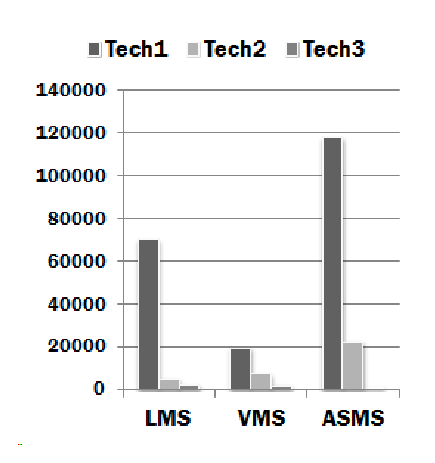
\includegraphics[width=2.0in]{test-rule.eps}
%        \vspace{-5pt}
%    \caption{\label{fig:framework} ACPT overview}
%    \vspace{-10pt}
%%    \vspace{+3pt}
%\end{figure}

%\begin{figure}[t]
%    \centering
%        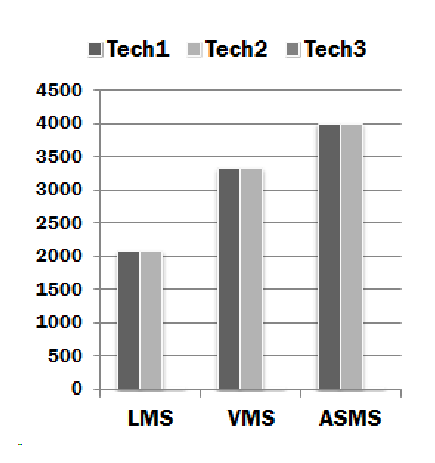
\includegraphics[width=2.0in]{testselection.eps}
%        \vspace{-5pt}
%    \caption{\label{fig:framework} ACPT overview}
%    \vspace{-10pt}
%%    \vspace{+3pt}
%\end{figure}





% Table generated by Excel2LaTeX from sheet 'Test Reduction'
%\begin{table*}[tbp]
%  \centering
%  \caption{Add caption}
%    \begin{tabular}{|r|r|r|r|r|r|rrrrrrrrrr}
%    \multicolumn{1}{c}{\multirow{2}[4]{*}{Subjects}} & \multicolumn{3}{c}{Regression - 5} & \multicolumn{3}{c}{Regression - 10} & \multicolumn{3}{c}{Regression - 15} & \multicolumn{3}{c}{Regression - 20} & \multicolumn{3}{c}{Regression - 25} & \\
%    \multicolumn{1}{c}{} & \# Counter & \# Covered & \% Covered & \# Counter & \# Covered & \% Covered & \# Counter & \# Covered & \% Covered & \# Counter & \# Covered & \% Covered & \# Counter & \# Covered & \% Covered \\
%    LMS   & 5.00  & 2.42  & 48.33 & 9.00  & 4.75  & 52.78 & 13.00 & 6.25  & 48.08 & 17.42 & 7.75  & 44.50 & 20.67 & 8.83  & 42.74 \\
%    VMS   & 4.92  & 0.42  & 8.47  & 9.25  & 0.67  & 7.21  & 13.83 & 1.33  & 9.64  & 18.92 & 1.08  & 5.73  & 23.75 & 1.75  & 7.37 \\
%    ASMS  & 5.00  & 1.92  & 38.33 & 9.75  & 4.75  & 48.72 & 14.42 & 7.33  & 50.87 & 18.67 & 9.42  & 50.45 & 23.33 & 12.08 & 51.79 \\
%    \end{tabular}%
%  \label{tab:addlabel}%
%\end{table*}%



\subsection{Subjects}
The subjects include three real-life Java programs each, which
interacts with access control policies \cite{mouelhi09:tranforming}. We next describe
our three subjects.
\begin{itemize}	
\item Library Management System (LMS) provides web services to manage books in a public library.
\item Virtual Meeting System (VMS) provides web conference services. VMS allows users to organize
online meetings in a distributed platform.
\item Auction Sale Management System (ASMS) allows users to buy or sell items on line. A seller initiates an auction by submitting a description of an item she wants to sell with its expected minimum price. Users then participate in bidding process by
bidding the item. For the bidding on the item, users have enough money in her account before bidding.
\end{itemize}

%Table~\ref{tab:subj} shows information in our subjects.
Our subjects use a Sun PDP \cite{sun05:xacml} to evaluate requests against a policy.
Sun PDP is popularly used PDP to evaluate requests.
Table~\ref{tab:subj} summarizes the basic statistics of our subjects. The first column shows the subject names.
Columns 2-5 show the lines of code (``LOC''), the numbers of total test cases (``\# Total''), security test cases (``\# Security Tests''),
rules covered with existing test cases (``\# Cov''), rules not-covered with existing test cases (``\# Not-Cov''), and the percentage
of rule coverage (``\% Cov''), respectively. For coverage, we refer rules are explicitly specified rules.
In addition, over all of existing test cases, we distinguish security test cases, which issue
more than one request to the PDP from test cases without interaction of policies.

Table~\ref{tab:subjectpolicies} summarizes the basic statistics of policies in our subjects.
The first column shows the subject names.
Columns 2-5 show the numbers of subjects, actions, resources, conditions, explicitly specified rules, implicit
 rules, and total rules for each policy.
The largest one consists of 129 rules.
For explicitly specified rules, developers first write rules for denying or permitting access
explicitly. Implicit rules refer to rules that are evaluated in a given policy, while the developers do not write such rules.
For example, In Figure~\ref{fig:example}, Line 34
specifies a rule. This rule denies all the requests $R_d$ that do not match with its preceding rules while
no rules (i.e., implicit rules) are specified to handle such requests explicitly.

\begin{table*}[htbp]
  \centering
  \caption{Coverage results of test cases selected for changed policy behaviors for each policy}
  	\vspace{-8pt}   
    \begin{tabular}{|l|r|r|r||r|r|r||r|r|r||r|r|r||r|r|r|}
%\multirow{2}{*}{Subject} & \multicolumn{3}{c}{Regression - 5} & \multicolumn{3}{c}{Regression - 10} & \multicolumn{3}{c}{Regression - 15} & \multicolumn{3}{c}{Regression - 20} & \multicolumn{3}{c}{Regression - 25} & \\
\hline
     \multirow{2}{*}{Subject} & \multicolumn{3}{|c||}{Regression - 5} & \multicolumn{3}{|c||}{Regression - 10} & \multicolumn{3}{|c||}{Regression - 15} & \multicolumn{3}{|c||}{Regression - 20} & \multicolumn{3}{|c|}{Regression - 25} \\\cline{2-16}
       & \# CT & \# Cov & \% Cov & \# CT & \# Cov & \% Cov & \# CT & \# Cov & \% Cov & \# CT & \# Cov & \% Cov & \# CT & \# Cov & \% Cov \\\hline\hline
    LMS   & 5.0   & 2.4   & 48.3  & 9.0   & 4.8   & 52.8  & 13.0  & 6.3   & 48.1  & 17.4  & 7.8   & 44.5  & 20.7  & 8.8   & 42.7 \\\hline
    VMS   & 4.9   & 0.4   & 8.5   & 9.3   & 0.7   & 7.2   & 13.8  & 1.3   & 9.6   & 18.9  & 1.1   & 5.7   & 23.8  & 1.8   & 7.4 \\\hline
    ASMS  & 5.0   & 1.9   & 38.3  & 9.8   & 4.8   & 48.7  & 14.4  & 7.3   & 50.9  & 18.7  & 9.4   & 50.4  & 23.3  & 12.1  & 51.8 \\\hline\hline
    Average & 4.97  & 1.58  & 31.71 & 9.33  & 3.39  & 36.23 & 13.75 & 4.97  & 36.19 & 18.33 & 6.08  & 33.56 & 22.58 & 7.56  & 33.97 \\\hline

    \end{tabular}%
  \label{tab:cov-results}%
\end{table*}%

%techniques as test selection based on mutation analysis ($Mut-Selection$)
%test selection based on coverage analysis ($Cov-Selection$)
%test selection based on recorded rrequest evaluation ($Req-Selection$)

% Table generated by Excel2LaTeX from sheet 'Performance'
\begin{table*}[htbp]
  \centering
  \caption{Elapsed time for each step of test selection technique, and each policy}
  	\vspace{-8pt}   
    \begin{tabular}{|l|r|r|r||r|r|r||r|r|}

			\hline
       \multirow{2}{*}{Subject}   & \multicolumn{3}{|c||}{Mut-Selection} & \multicolumn{3}{|c||}{Cov-Selection} & \multicolumn{2}{|c|}{Req-Selection} \\\cline{2-9}

%          & Pre-computed & \multicolumn{2}{c}{Post-computed} & Pre-computed & \multicolumn{2}{c}{Post-computed} & Pre-computed & Post-computed \\\cline{2-7}
          & TEST-Rule & CIA & Test Selection & TEST-Rule & CIA& Test Selection & Req Collection & Test Selection \\\hline\hline
%    LMS   & 70496 & 2083.333333 & 4.25  & 5214  & 2083.333 & 4.25  & 2096  & 1.933333 \\\hline
%    VMS   & 19771 & 3333.333333 & 0.766667 & 7506  & 3333.333 & 0.766667 & 1873  & 1.866667 \\\hline
%    ASMS  & 118248 & 4000  & 11.36667 & 22423 & 4000  & 11.36667 & 1064  & 20.7 \\\hline

		LMS   & 70496 & 2083  & 4     & 5214  & 2083  & 4     & 2096  & 2 \\\hline
    VMS   & 19771 & 3333  & 1     & 7506  & 3333  & 1     & 1873  & 2 \\\hline
    ASMS  & 118248 & 4000  & 11    & 22423 & 4000  & 11    & 1064  & 21 \\\hline\hline
    Average & 69505 & 3139  & 5     & 11714 & 3139  & 5     & 1678  & 8 \\\hline

    
    \end{tabular}%
  \label{tab:performance-results}%
\end{table*}%

\subsection{Objectives and Measures}
In the evaluation, we intend to answer the following research questions:
\begin{itemize}


	\item RQ1: How many of test cases in a test suite (from an existing test suite) selected by our test selection techniques? This question helps to show that our techniques can reduce a significant number of test cases in an existing test suit.
	We also show how many changed policy behaviors are covered with our selected test cases.
	
%	\item RQ2: Do our protest selections are safe? This question helps to show that our techniques select all tests, which shows only and all test cases to reveal changed behaviors in access control policies.
	
	\item RQ2: What are elapsed time for our techniques to conduct test selection by given subjects? This question helps to compare performance of our techniques by measuring efficiency with regards to elapsed time.
			
	\item RQ3: How higher we can achieve additional policy coverage ratio by our test augmentation technique?  This question helps to show that our technique can generate/augment test suite to cover 100\% of changed policy behaviors. We also compare our approach with random test generation technique to show how effectively our approach augment test suite to cover not-coverted changed policy behaviors.
				
\end{itemize}

%\subsection{Metrics}
%
%We use following 4 metrics in our evaluation.
%\begin{itemize}
%	\item Policy coverage information for changed policy behaviors.
%	\item Number of test cases reused by the test selection technique.
%	\item Elapsed time of test-rule correlation, change impact analysis, and test selection.
%	\item Number of test cases generated by the test augmentation technique. 
%\end{itemize}




\begin{figure}[htbp]
    \centering
        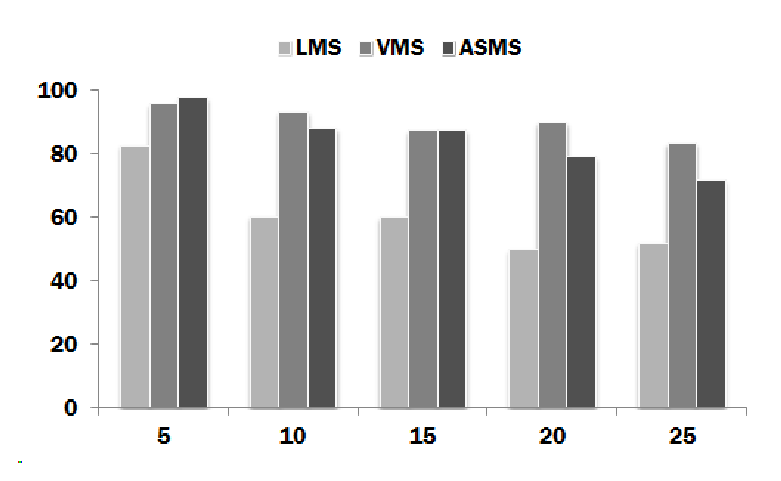
\includegraphics[width=3.0in]{reduction.eps}
        \vspace{-5pt}
    \caption{\label{fig:reduction} Regression test selection results (test reduction) for our subjects and each modified version. Y axis
    denotes the percentage of test reduction. X axis denote the number of policy changes in modified policy of our subjects.}
    \vspace{-10pt}
%    \vspace{+3pt}
\end{figure}



\subsection{Results}
To answer $RQ1$, 
we measure how many test cases are reduced for regression testing.
The goal of this research question is to show the reduction in the number of test cases that
are selected using our techniques. The reduction in the number
of test cases is the same across our three techniques.
Figure~\ref{fig:reduction} shows the results of test reduction for the three subjects.
We observe that 82\%$\sim$97\% of test reduction for a modified version with 5 policy changes.
We observe that 51\%$\sim$83\% of test reduction for a modified version with 25 policy changes.
Such test reduction may reduce a significant cost in terms of test execution time
for regression testing. We found that all of our test techniques show the same
set of selected test cases to show that all of our techniques can detect every
test case impacted policy changes.

To answer $RQ2$, we measure how many test cases are reduced for regression testing.
The goal of this research question is to compare performance of our three
test selection techniques.
Table~\ref{tab:performance-results} shows the results, which is elapsed time for the three subjects and
each technique.
For $Mut$-$Selection$ and $Cov$-$Selection$, the table shows the elapsed time of
test-rule correlation (``Test-Rule''), change-impact-analysis (``CIA''), and test
selection (``Test Selection''), respectively.
For $Req$-$Selection$, the table shows the elapsed time of
request recording (``Req-Collection''), and test
selection (``Test Selection'').
Note that ``Test-Rule'' and ``Req-Collection'' are preliminary step that could
be done before test selection. 
We observe that $Cov$-$Selection$ (11,714 milliseconds on average) a significant
elapsed time compared to $Mut$-$Selection$ (on average 69505 milliseconds) in terms of test-rule correlation.
Moreover, we observe that a total elapsed time of $Req$-$Selection$ is 43 and 8 times
faster than those of $Mut$-$Selection$  and $Cov$-$Selection$, respectively.


%$Mut$-$Selection$ and $Cov$-$Selection$ show
%elapsed time 69505 (mm) and 11714 (mm) for test-rule correlation.
% $Cov$-$Selection$  


%the reduction in the number of test cases that
%are selected using our techniques.
%
%To measure the efficiency of our three techniques, we conducted evaluation as follows. 
%We compared elapsed time to analyze test-rule correlation analysis,
%change impact analysis, and test selection by each technique.
%For the first two techniques, we require test-rule correlation analysis
%and change impact analysis, which should be done before actual test selection.
%The objective of this evaluation is to investigate how our three test selection techniques impacts performance for subjects.



Table~\ref{tab:cov-results} shows the coverage results of selected test cases for the three subjects.
For each subject, the table shows the number of
changed policy behaviors (``\# CT''), test
cases that were selected (``\# Cov''), and the percentage of test
cases that were selected (``\% Cov'') for each version of its policy.
We denote our modified version of a policy as ``Regression - N'' where
$N$ denotes the number of changes injected into the policy.
``\# CT'' is equal or less than $N$ because our injected changes may not introduce
policy behavior changes at the final modified version of the policy. For example, if one changes
one rule with $CRE$ and again changes the rule with $CRE$. As the results, the rule does not impact
on policy changes.



% Table generated by Excel2LaTeX from sheet 'test augument'
\begin{table}[htbp]
  \centering
  \caption{Test case type ratios of augmented test cases for our subjects}
    \begin{tabular}{|l|r|r|r|r|}
		\hline
    Subjects & \% M-Sub & \% M-Cond & \% M-SubCond  & \% Others \\\hline\hline
    LMS   & 21.83 & 4.93  & 11.27 & 61.97 \\\hline
    VMS   & 3.41  & 0.38  & 1.89  & 94.32 \\\hline
    ASMS  & 16.30 & 9.63  & 7.41  & 66.67 \\\hline\hline
    Average & 13.85 & 4.98  & 6.86  & 74.32 \\\hline
    \end{tabular}%
  \label{tab:augment-results}%
\end{table}%
 \vspace{-20pt}
\begin{figure}[htbp]
    \centering
        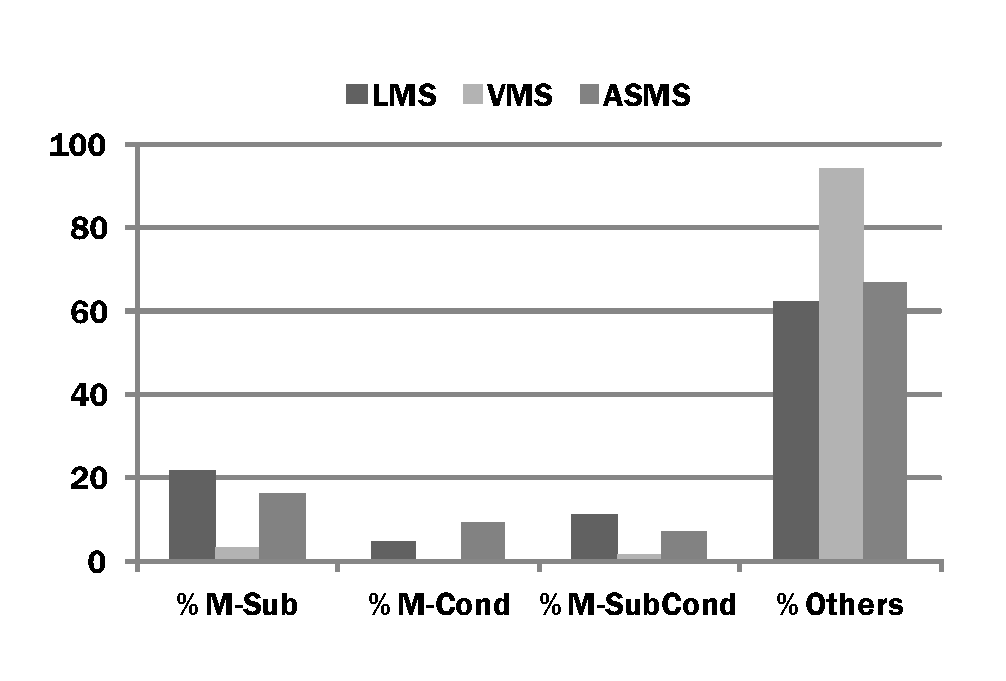
\includegraphics[width=3.0in]{augmenttypes.eps}
        \vspace{-5pt}
    \caption{\label{fig:augment-results} Augmented test results for our subjects and each modified version. Y axis
    denotes the percentage of augmented test cases. X axis denote the types of the augmented test cases.}
    \vspace{-10pt}
%    \vspace{+3pt}
\end{figure}

%[TBD:Results-test augmentation]

To answer $RQ3$, we first identify
changed policy behaviors (i.e., rules impacted by policy changes), which
are not-covered with existing test cases.
Note that existing test cases cannot reveal faults introduced by such policy behaviors.
In Table~\ref{tab:cov-results}, we observe that our selected test cases
cover 31.71$\sim$36.23\% of changed policy behaviors. The result show
that about 70\% of changed policy behaviors (i.e., rules impacted by policy changes) are not-covered.
We apply our test augmentation technique to add new test cases
to cover such not-covered-rules.

Table~\ref{tab:augment-results} shows the results of test augmentation for the three subjects.
When developers know which policy behaviors to cover, the developers could generate
test cases with requests to cover the policy behaviors. 

For each subject, the table shows the percentage of
generated test cases for each argumentation type type defined in Section~\ref{subsec:testaugmentation}.
%$[\frac{a}{b}]$ 
While we generate/modify test cases to cover 100\% percentage of not-covered
policy behaviors, we may augment test cases based on following different types of modification/generation.
``M-Sub'' refers to generate test cases by modifying
subject elements in test cases. For example, Given test cases, by changing subject elements (e.g,
BORROWER instead of SECRETARY),
the test cases cover the changed behaviors, which was not-covered in existing test cases
shown in Table~\ref{tab:augment-results}.
Similarly, ``M-Cond'' refers to generate test cases by modifying
condition elements in test cases.
When two of the preceding modification could not
find test cases to modify, our technique finds
``M-SubCond'', which refers to generate test cases by modifying
subject elements and condition elements together.
At the last column, ``Others'' denotes an argumentation type, which
may at least change action and resource elements.

In Table~\ref{tab:augment-results}, we observe that
a total of 26\% of the augmented test cases are modified by
existing test cases in columns 2,3, and 4. However,
for more than 74\% of the augmented test cases are
generated by scratch since we could not find similar
test cases.
Figure~\ref{fig:augment-results} illustrated
the same data shown in Table~\ref{tab:augment-results}.

By comparing these results with those in Table~\ref{tab:cov-results}, we observe that there is indeed a correlation between coverage and 
test augmentation.
The higher percentage of rule coverage for each subject,
the higher percentage of tests are augmented
by the first three types with modifying subject
or condition elements.
The reason is that, if the subject has test cases with high rule coverage, it is likely
to find similar test cases to modify than subjects with test cases with low rule coverage.

\subsection{Threats to Validity}
The threats to external validity primarily include the degree to
which the subject programs, the policies and regression model are representative of true practice.
These threats
could be reduced by further experimentation on a wider type of policy-based software systems and
larger number of policies.
In particular, our proposed regression model based on \CodeIn{RMR}, \CodeIn{RA},
and \CodeIn{CRE} modifies policy elements such as subject, resource, action, and condition attributes.
Additional regression model to modify various policy attributes could
simulate various policy modification.
The threats to internal validity are instrumentation effects
that can bias our results such as faults in Sun's PDP, faults in Margrave, and
faults in our implementation.


\section{Discussion}\label{sec:discussion}
We believe that our approach can be applied to select
test cases in programs each interacting
with policies written in languages (such as EPAL~\cite{epal} and Alloy~\cite{jackson01:micromodularity}) other than XACML.
For policies written in other languages, we could evaluate test cases or requests issued from test cases
to set up test-rule correlation or capture requests. 
As our approach requires change impact analysis (against a policy and
its modified policy) provided by the existing policy change impact tool to adopt
XACML policies, we could convert the policies to XACML policies
while maintain semantics of policies for change impact analysis.


%such conversion enables our approach to also be applicable to policies languages other than XACML and with veri?cation
%tools other than Margrave.


%a
%ssess
%the quality of a property set against policies written in languages other than XACML. Previous approaches converted
%policies in one language (such as XACML) to other languages (such as Alloy [12], RW [23], and Description Logics [14]) that are equipped with veri?cation tools. As our
%approach requires property veri?cation (against a policy and
%its mutants) provided by these veri?cation tools, such conversion enables our approach to also be applicable to policies languages other than XACML and with veri?cation
%tools other than Margrave.
%Our approach to mutation veri?cation provides a quality assessment of a property set for a policy. If a property
%set achieves a mutant-killing ratio of 100%, can we say that
%the property set is exhaustive or complete? This situation is
%similar to statement coverage in software testing. If a test
%suite achieves 100% statement coverage for a given program, can we say the test suite can detect all faults in the
%program? The answer, of course, is absolutely not. While
%mutation veri?cation serves as a quality assessment for a


%\textbf{
%One example is the conference policy; the structural
%coverage for the two random request sets is zero and, as expected,
%the mutant-killing ratio is also zero. Similarly we observe that
%the mutant-killing ratios across all subjects for the random and
%selected random request sets are quite similar. Unfortunately the
%mutant-killing ratio is still low when considering the high structural coverage.}


%The same data is illustrated in Figure 4
%, ``\% M-Cond'', ``\% M-SubCond'', and ``\% Others''
%refer to four test argumentation type 


%number of
%changed policy behaviors (``\# CT''), test
%cases that were selected (``\# Cov''), and the percentage of test
%cases that were selected (``\% Cov'') for each version of its policy.
%We denote our modified version of a policy as ``Regression - N'' where
%$N$ denotes the number of changes injected into the policy.
%``\# CT'' is equal or less than $N$ because our injected changes may not introduce
%policy behavior changes at the final modified version of the policy. For example, if one changes
%one rule with $CRE$ and again changes the rule with $CRE$. As the results, the rule does not impact
%on policy changes.

%selects test cases
%
%
%DT , Basic and P rioritization
%detect averagely 25.9%, 62.3%, and 62.3% 


%changes may not lead to.



%The data in the gure illustrate that the reduction in the
%number of selected test cases varies widely both across and
%within the subjects.


%techniques as test selection based on mutation analysis ($Mut$-$Selection$)
%test selection based on coverage analysis ($Cov$-$Selection$)
%test selection based on recorded rrequest evaluation ($Req$-$Selection$)


%Test Suite Reduction. The goal of this study was
%to determine the reduction in the number of test cases that
%could be achieved using our regression-test-selection tech-
%nique. For each subject program P, and each version P',
%we used Retest, shown in Figure 8, to select test cases for
%regression testing.


%
%For each subject, the gure shows the percentage of test
%cases that were selected for each version of that subject.
%The data in the gure illustrate that the reduction in the
%number of selected test cases varies widely both across and
%within the subjects.
%
%Study 2: Safe --------
%
%Whether this result is safe or not. We also compute empirically,
%test dependency and failed together. Okay.
%
%Study 3: Performance ------------ Graph.
%we show that, our testing results is good.
%
%Study 4: augumentation
%
%
%
%	
%[ToDo: explain more]

% Table generated by Excel2LaTeX from sheet 'Sheet1'


%Metrics # of code
%Metrics # of rules in a policy
%Metrics # of system tests
%	seucrity tests
%	selected tests


%In our evaluation, we measure request processing time by evaluating randomly
%generated requests developed by our previous work~\cite{Xengine}.
%In particular, for multiple PDPs, our approach fetches a PEP with a corresponding
%PDP for a given request at run time. Therefore, request processing time includes
%both fetching time and request evaluation time.


%\begin{figure*}[h!]
%  \centering
%  \subfloat[LMS]{\label{fig:gull}\includegraphics[width=0.33\textwidth]{LMS.pdf}}                
%  \subfloat[VMS]{\label{fig:VMS}\includegraphics[width=0.33\textwidth]{VMS.pdf}}
%  \subfloat[ASMS]{\label{fig:ASMS}\includegraphics[width=0.33\textwidth]{ASMS.pdf}}
%  \caption{Request Processing Time for our subjects LMS, VMS and ASMS}
%  \label{fig:processing time}
%\end{figure*}

%\subsection{Performance Improvement Results}\label{subsec:performanceimprovement}
%
%We generated the resulting sub-policies for all the splitting criteria defined in Section~\ref{subsec:SplittingCriteria}.
%For each splitting criteria, we have conducted systems tests to generate requests that trigger all the PEPs in the evaluation. 
%The test generation step leads to the execution of all combination of possible requests described in our previous work \cite{testcase}.  
%The process of tests generation is repeated for ten times in order to avoid the impact of randomness.
%We applied this process to each splitting criterion and calculated evaluation time on average of a system under tests.



\section{Related Work}
\label{sec:related}


Various techniques have been proposed on regression testing of software programs in software engineering and
programming language communities~\cite{Rothermel:1996:ART:235681.235682, Graves:2001:ESR:367008.367020, cite{Elbaum:2000:PTC:347324.348910,santelices08sep}}.
These techniques aim to select every test case to reveal different behaviors correctly after modification
in program or augment test cases.
These techniques are related to regression test selection \cite{Rothermel:1996:ART:235681.235682}, 
\cite{Graves:2001:ESR:367008.367020}, test-suite prioritization \cite{Elbaum:2000:PTC:347324.348910}, and test-suite augmentation \cite{santelices08sep}. 
Note that these techniques focus on changes at code level.
None of these techniques consider potential changes that can arise from code-related components (such as a policy that interacts with application code).
Polices and general programs are fundamentally different in terms of structures, semantics, and
functionalities, etc. Therefore, techniques for regression
testing of general programs are not suitable for addressing 
the test selection problem for policy evolution.
Our work is the first one for automatic test-selection approach in context of policy
evolution.

Prior work that is closest to ours is Mouelhi et al.��s
work~\cite{mouelhi09:tranforming}.
They proposed a technique to transform functional test cases into security test cases. 
These test cases then be used to verify correctness of access control mechanisms in policy-based systems.
They defined various mutation operators at the policy level.
Given a policy and its mutated policy, the technique selects only impacted test cases to be transformed security test cases
(with additional manual task to add code for security check).
While this work focuses on security test case selection from initial test cases,
our work focuses on test selection problem impacted by policy changes
to reveal faults induced by policy changes.

Another work closest to ours is Fisler et al.��s
work~\cite{Fisler:2005:VCA:1062455.1062502}.
They developed a tool called ``Margrave'' that enables verifying properties against 
policies written in XACML and conduct change impact analysis. Margrave is based on multi-terminal binary decision diagrams and allows several forms of 
constraints to be added as properties in the Scheme programming language.
While Margrave is effective to detect changed policy behaviors between two versions
of a policy specified in XACML at policy level, Margrave does not handle with situations where
program behaviors are changed by policy changes as our work fouces on.

%in terms of regression testing. As application
%code can often interact with policies, our work is useful

To facilitate verifying and validating the correctness of policies, prior
research work has been done in the area of policy testing, which generates and executing test requests against a policy.
Martin et al. ~\cite{martin06:defining} proposed a framework to detect policies faults by analyzing
policy test suites that involve 
requests-responses pairs. The framework is based on mutation operators ~\cite{martin07:fault} that enable measuring fault detection capability. 
It uses a tool \cite {martin07:automated} that aims at minimizing the test cases to be generated by analyzing the structural coverage of the policies.
Hu et al. ~\cite{hu07:conformance} proposed a generic model-based conformance checking technique for access control policies written in
XACML.
These approaches focus on test request generation at a policy level (e.g., policies written in XACML).
Instead of generating new requests, our work focuses on regression testing at the implementation level (the system level) by
reusing existing hardcoded test cases.
%, which includes
%application code when a policy evolves. 


%Margrave detects the presence of requests that may violate the specified properties.

%used these mutated policies to select impacted tests. The impacted tests are then tranformed to security tests (by added specific code to check the security mechanism). 
%Although this work focused on applications interacting with policies, it was not presented from a regression testing perspective.
%
%
%The most relevant paper that is related to our work was presented by Mouelhi et al. in~\cite{mouelhi09:tranforming}. The authors proposed transforming functional tests into security tests. 
%These tests can then be used to validate the access control mechanisms in policy-based systems. They defined mutation operators at the policy level and used these mutated policies to select impacted tests. The impacted tests are then tranformed to security tests (by added specific code to check the security mechanism). 
%Although this work focused on applications interacting with policies, it was not presented from a regression testing perspective. 

%fault
%localization problem of ?rewall policies.
%
%This paper focuses on regression testing for policy-based software systems.

 


%Zhang et al \cite{DBLP:conf/isw/ZhangRG05} used model checking technique which is supported by a tool to evaluate access
%control policies specified in a modelling formalism called RW. Hughes et al. \cite{hughes04:automated} proposed using First-Order Logic 
%to automatically verify access control policies. Their model is based on specifying access to resources, they show that the access
%control policies in XACML can be translated into a normlized form that includes four classes: permit,
%deny, error, and not-applicable. A partial ordering among access control polices enable the authors to specify properties that are checked later
%with Alloy analyszer \cite{Alloy}. Nyanchama et. al. \cite{Nyanchama99therole} focused on policy analysis and verification related to 
%RBAC models. They used graphs to model hierarchies of users, roles and permissions and to solve role-role conflicts issues.
%While these different approaches focus on test request generation for validating the policy implementation (the XACML code), 
%the technique presented in this paper focuses on regression testing at the implementation level (the system level) which occurs when the access control policy evolves. 





\Comment{
Our previous work~\cite{hu10:model,hu08:property} presented
model checking to verify various policies such as role-based
access control policies~\cite{ferraiolo92:role}.
Our previous work translates policies into specifications
in NuSMV~\cite{cimatti02:nusmv2}. NuSMV verifies the specifications against properties. 
Based on our previous work, we developed a tool, called ACPT\footnote{http://csrc.nist.gov/groups/SNS/acpt/index.html},
to verify and test access control policies.
However, our previous work does not detect conflicts
or redundancies between two policies, one major
focus of our current work. Moreover, our previous
work does not recommend any combinations (to the policy
authors) that can be recommended by our current work. 

There exist tools to verify XACML policies. These tools require XACML policies in formal specification languages such as 
Alloy~\cite{jackson01:micromodularity}. Hughes et al.~\cite{hughes04:automated} proposed an approach to translate XACML policies to a model 
specified in the Alloy language~\cite{jackson01:micromodularity}. Then, the Alloy Analyzer verifies whether the model satisfies the given properties.
Kolovski et al.~\cite{kolovski07:analyzing} converted XACML policies into specifications in  description logics (DL) and adopted existing DL 
verification tools to verify the specifications. Fisler et al.~\cite{fisler05:verification} developed a Binding Decision Diagram (BDD) based 
verification tool, called Margrave, to verify XACML policies. Margrave parses XACML policies into the BDD structure. Moreover, Margrave supports 
change-impact analysis to report which decisions are changed after policy modification.
Similar to these previous approaches, our approach focuses on modeling and verifying policies via a symbolic model checking. Moreover, our approach
 verifies whether two policies may include conflicts and redundancies via a symbolic model checking. 
While these previous approaches do not help combining two policies, our approach recommends combinations of two policies that could satisfy 
user-specified properties. 


%\textbf{Policy Combinations/Integration.}
%Bonatti et al.~\cite{Bonatti2} proposed combining sub-policies based on 2-valued algebra. 
Backes et al.~\cite{backes04algebra} proposed a 3-valued algebra to combine sub-policies considering privacy policies.
 They defined relations of combination with three operators: conjunction, disjunction, and scoping.
 Li at el.~\cite{Ninghui2009} proposed an algebra for combining sub-policies. 
They introduced new combining algorithms such as weak majority or strong majority.
For example, in the case of the strong majority combining algorithms, at least 2/3 
rules evaluated against a request should be evaluated to the same decision. Since the decision is the majority, 
the decision is returned as a final decision. They proposed algebras to generalize their combining algorithms.
%Mazzoleni et al.~\cite{Mazzoleni2006} proposed policy integration that can be applied to XACML policies. 
In their approach, policy authors can specify conditions to represent how their policies can be integrated with other policies. 
Their integration approach is based on analysis of two policies to be integrated. Policy authors measure similarity of two policies 
and integrate the policies based on given condition.





}
\Comment{
%\textbf{Policy Change Impact Analysis}
%\textbf{Policy Conflict and Redundancy}
%\textbf{Verification in NuSMV for other projects}

%interaction, but runtime ...more general stuff to do it.

\textbf{Policy Verification.}
There are verification tools available for XACML
policies. Hughes et
al.~\cite{hughes04:automated}
proposed an approach
to verify XACML policies by
translating the policies to the Alloy
language~\cite{jackson01:micromodularity}.
Then, they use Alloy Analyze to verify properties
against the translated policies. 
Zhang et
al.~\cite{zhang05:evaluating} developed a model-checking tool
to verify policies specified in
\Intro{RW} languages~\cite{zhang04:synthesis}, which can be converted to
XACML.
Kolovski et
al.~\cite{kolovski07:analyzing} formalize XACML policies with
description logics (DL), which are a decidable fragment of
first-order logic, and exploit existing DL verifiers to conduct
policy verification.
Schaad and Moffett~\cite{schaad02:lightweight} leverage
Alloy~\cite{jackson01:micromodularity} to check that role-based
access-control policies do not allow roles to be assigned to users
in ways that violate SoD constraints.
Similar to previous research work, our work also model and verify policies
via model checking. However, we extend
our work to detect conflict and redundancy via a symbolic checker.


\textbf{Policy Combinations/Integration.}
Bonatti et al.~\cite{Bonatti2} proposed combining sub-policies based on 2-valued algebra. Backes et al.~\cite{backes04algebra} proposed a 3-valued algebra to combine sub-policies considering privacy policies. They defined relations of combination with three operators: conjunction, disjunction, and scoping. Li at el.~\cite{Ninghui2009} proposed an algebra for combining sub-policies. They also introduce new combining algorithms such as weak majority or strong majority. For example, in case of the strong majority combining algorithms, at least 2/3 rules evaluated against a request should return the same decision. As the decision is majority, the decision is returned as a final decision. They propose algebras to generalize their combining algorithms. Moreover, they propose combinations of sub-policies, which may return policy evaluation errors and obligations.
Mazzoleni et al.~\cite{Mazzoleni2006} proposed policy integration that can be applied to XACML policies. In their approach, policy authors can specify conditions to represent how their policies can be integrated with other policies. Their integration approach is based on analysis of two policies to be integrated. Policy authors measure similarity of two policies and integrate the policies based on given condition.
We also propose that a methodology to combine two policies using property verification.
We next describe a methodology to recommend the combinations (of two policies) that could satisfy user-specified properties.

\textbf{Policy Testing.}

Our previous work~\cite{hu10:model} demonstrated an approach
to represent a policy and its properties as
corresponding finite state machine (FSM) model and temporal
logics (e.g., computation tree logic), respectively, using SMV specification language~\cite{cimatti02:nusmv2}.

Our previous work developed policy testing approaches for policy
structural coverage~\cite{martin06:defining}, request
generation~\cite{martin07:automated}, and mutation
testing~\cite{martin07:fault}.
% Our previous
%work~\cite{hu07:conformance} also proposed a generic model-based
%conformance checking approach for access control policies written in
%XACML.
These pieces of work do not rely on properties for generating
test requests to detect a fault in a policy. 
Our previous work~\cite{martin08:assessing} developed an approach
for measuring the quality of policy properties in policy
verification. Given user user-specified
properties, the quality of properties are measured
based on fault-detection capability.
}
\section{Conclusion}
\label{sec:conclusion}

We make three key contributions in this paper. First, we
proposed a test selection approach for
access control policy evolution.
To the best of our knowledge,
our paper is the first one for automatic test-selection approach in context of policy
evolution.
We present three automatic test-selection techniques.
Second, we presented a test augmentation technique to
select test cases for modification to cover not-covered
policy changes. Third, we conduct
evaluation with three metrics
to measure the effectiveness of our approach
and the efficiency of our three test selection
techniques.
The evaluation results demonstrated that our approach is effective to select
test cases for test reduction.
Among the proposed three test-selection techniques, the evaluation results demonstrated that the technique based recorded
request evaluation is the most efficient compared with other
two techniques. Besides, we also achieve 100\% coverage
of changed policy behaviors with augmented test cases.


%the first
%  and the second techniques in terms of elapsed time. 


%If 
%
%generate additional new test cases to cover not-covered-impacted-rules with selected test cases by the preceding techniques.
%
%to select every test case impacted by policy changes.
%
%
%from existing test cases to test program code impacted by policy changes.
%
%comprehensive fault model for ?rewall
%policies, including ?ve types of faults. For each type of
%fault, we present an automatic correction technique. Second, we propose the systematic approach that can automatically correct all or part of the misclassi?ed packets
%of a faulty ?rewall policy. To the best of our knowledge,
%our paper is the ?rst one for automatic correction of ?rewall policy faults. Last, we implemented our approach
%and evaluated its effectiveness on real-life ?rewalls. To
%measure the effectiveness of our approach, we propose
%two metrics, which we believe are general metrics for
%measuring the effectiveness of ?rewall policy correction
%tools. The experimental results demonstrated that our approach is effective to correct a faulty ?rewall policy with
%three types of faults:
%
%Conclusion here!!


%ACKNOWLEDGMENTS are optional
%\section{Acknowledgments}
%This section is optional; it is a location for you
%to acknowledge grants, funding, editing assistance and
%what have you.  In the present case, for example, the
%authors would like to thank Gerald Murray of ACM for
%his help in codifying this \textit{Author's Guide}
%and the \textbf{.cls} and \textbf{.tex} files that it describes.

%
% The following two commands are all you need in the
% initial runs of your .tex file to
% produce the bibliography for the citations in your paper.
\bibliographystyle{abbrv}
\bibliography{yangtse,yangtse2}  % sigproc.bib is the name of the Bibliography in this case
% You must have a proper ".bib" file
%  and remember to run:
% latex bibtex latex latex
% to resolve all references
%
% ACM needs 'a single self-contained file'!
%
%APPENDICES are optional
%\balancecolumns
%\appendix
%%Appendix A
%\section{Headings in Appendices}
%The rules about hierarchical headings discussed above for
%the body of the article are different in the appendices.
%In the \textbf{appendix} environment, the command
%\textbf{section} is used to
%indicate the start of each Appendix, with alphabetic order
%designation (i.e. the first is A, the second B, etc.) and
%a title (if you include one).  So, if you need
%hierarchical structure
%\textit{within} an Appendix, start with \textbf{subsection} as the
%highest level. Here is an outline of the body of this
%document in Appendix-appropriate form:
%\subsection{Introduction}
%\subsection{The Body of the Paper}
%\subsubsection{Type Changes and  Special Characters}
%\subsubsection{Math Equations}
%\paragraph{Inline (In-text) Equations}
%\paragraph{Display Equations}
%\subsubsection{Citations}
%\subsubsection{Tables}
%\subsubsection{Figures}
%\subsubsection{Theorem-like Constructs}
%\subsubsection*{A Caveat for the \TeX\ Expert}
%\subsection{Conclusions}
%\subsection{Acknowledgments}
%\subsection{Additional Authors}
%This section is inserted by \LaTeX; you do not insert it.
%You just add the names and information in the
%\texttt{{\char'134}additionalauthors} command at the start
%of the document.
%\subsection{References}
%Generated by bibtex from your ~.bib file.  Run latex,
%then bibtex, then latex twice (to resolve references)
%to create the ~.bbl file.  Insert that ~.bbl file into
%the .tex source file and comment out
%the command \texttt{{\char'134}thebibliography}.
%% This next section command marks the start of
%% Appendix B, and does not continue the present hierarchy
%\section{More Help for the Hardy}
%The acm\_proc\_article-sp document class file itself is chock-full of succinct
%and helpful comments.  If you consider yourself a moderately
%experienced to expert user of \LaTeX, you may find reading
%it useful but please remember not to change it.
\balancecolumns
% That's all folks!
\end{document}
